%%%%%%%%%%%%%%%%%%%%%%%%%%%%%%%%%%%%%%%%%%%%%%%%%%%%%%%%%%%%%%%%%%%%%%%%%%%%%
%   EnICS Templates: template selector (for the template maintainer)
%
%   In the template project, this file just points at one of the templates
%   under the Templates folder, so that any of them can be compiled quickly.
%
%   TO START YOUR OWN MANUSCRIPT, do NOT edit this file. Instead, make the
%   template you need your main.tex:
%       1. Delete this main.tex
%       2. Move Templates/<the one you want>.tex to the root of the project
%       3. Rename it main.tex
%   That is it. Overleaf keeps compiling main.tex, and the whole body of your
%   manuscript lives in the root of the project.
%   (Or open the project with Claude Code and ask to "start a new EnICS manuscript".)
%
%   See README.md for the full tour.
%%%%%%%%%%%%%%%%%%%%%%%%%%%%%%%%%%%%%%%%%%%%%%%%%%%%%%%%%%%%%%%%%%%%%%%%%%%%%

% For IEEE Journal
\documentclass[journal]{IEEEtran}
%%%%%%%%%%%%%%%%%%%%%%%%%%%%%%%%%%%%%%%%%%%%%%%%%%%%%%%%%%%%%%%%%%%%%%%%%%%
%   EnICS Templates: IEEE Journal (IEEE Transactions) manuscript
%   To start writing: make this file the main.tex in the root of the project
%   (see README.md, or ask Claude to "start a new EnICS manuscript").
%%%%%%%%%%%%%%%%%%%%%%%%%%%%%%%%%%%%%%%%%%%%%%%%%%%%%%%%%%%%%%%%%%%%%%%%%%%

%%%%%%%%%%%%%%%%%%%%%%%%%%%%%%%%%%%%%%%%%%%%%
%    EnICS Templates: version stamp
%%%%%%%%%%%%%%%%%%%%%%%%%%%%%%%%%%%%%%%%%%%%%
% Bump this when releasing a new version of the templates to GitHub.
% Derived projects carry it, so anyone can tell which template version they started from.
\newcommand{\enicstemplateversion}{2026.09}

%%%%%%%%%%%%%%%%%%%%%%%%%%%%%%%%%%%%%%%%%%%%%
%    Don't warn me about loading packages
%%%%%%%%%%%%%%%%%%%%%%%%%%%%%%%%%%%%%%%%%%%%%
\usepackage{silence}

%%%%%%%%%%%%%%%%%%%%%%%%%%%%%%%%%%%%%%%%%%%%%
%    Template guidance switch
%%%%%%%%%%%%%%%%%%%%%%%%%%%%%%%%%%%%%%%%%%%%%
% All explanatory (colored) text in the templates is conditional on \ifguide.
% Each template sets \guidetrue in its preamble; change it to \guidefalse
% to remove every piece of guidance from the PDF at once.
\newif\ifguide
    \guidetrue

%%%%%%%%%%%%%%%%%%%%%%%%%%%%%%%%%%%%%%%%%%%%%
%    Variables per conference/journal
%%%%%%%%%%%%%%%%%%%%%%%%%%%%%%%%%%%%%%%%%%%%%
% All variables are false by default. Each template turns on the one(s) it needs.

% For Research Proposal template specific configurations
\newif\ifproposal
    \proposalfalse

% For Thesis template specific configurations
\newif\ifthesis
    \thesisfalse

% For IEEE Journal template specific configurations
\newif\ifieeejournal
    \ieeejournalfalse
% For ACM Journal template specific configurations
%     based on the template found here: https://www.acm.org/publications/authors/submissions
\newif\ifacmjournal
    \acmjournalfalse
% For adding author biographies
\newif\ifbiographies
    \biographiesfalse
% For adding a reply to reviewers
\newif\ifreplytoreviewers
    \replytoreviewersfalse

% For IEEE Conference template specific configurations
\newif\ifieeeconference
    \ieeeconferencefalse

% For ISF template specific configurations
\newif\ifisf
    \isffalse

% For ACM Conference (MICRO) template specific configurations
\newif\ifmicro
    \microfalse

% For template specific configurations
% \newif\if
%     \false

    \ieeejournaltrue        % IEEE Journal specific configurations
    \biographiestrue        % Add author biographies at the end of the paper
    \replytoreviewerstrue   % Append the reply-to-reviewers letter (Reply_To_Reviewers.tex)
    \guidetrue              % Show the template guidance text. Change to \guidefalse to hide all of it.

\usepackage{packages/basic_packages}
\input{packages/macros}
\input{newcommands/units}
%=================================%
% 	    	GLOSSARY       	      %
%   Common Acronyms & Commands    %
%=================================%
% \gls{formula}   -> singular -> e.g: formula 
% \Gls{formula}   -> singular + capital letter -> e.g: Formula 
% \glspl{formula} -> plural -> e.g: formulas 
% \Glspl{formula} -> plural + capital letter -> e.g: Formula
%
%   \newacronym{}{}{}
%   \newcommand{\}{}
\newacronym{sota}{SoTA}{state-of-the-art}
    \newcommand{\sota}{\gls{sota}\xspace}
\newacronym{iot}{IoT}{internet-of-things}
    \newcommand{\iot}{\gls{iot}\xspace} 
    \newcommand{\Iot}{\Gls{iot}\xspace} 
\newacronym{snr}{SNR}{signal-to-noise ratio}
    \newcommand{\snr}{\gls{snr}\xspace}
\newacronym{ppa}{PPA}{performance, power, and area}
    \newcommand{\ppa}{\gls{ppa}\xspace}
\newcommand{\var}{$\sigma/\mu$\xspace}
\newcommand{\std}{$\sigma$\xspace}

\newacronym{cdf}{CDF}{cumulative distribution function}
\newacronym{pdf}{PDF}{probabililty distribution function}
\newacronym{ip}{IP}{intellectual property}
\newacronym{fir}{FIR}{finite impulse response}
\newacronym{dsp}{DSP}{digital signal processing}
\newacronym[longplural={central processing units}]{cpu}{CPU}{central processing unit}
    \newcommand{\cpu}{\gls{cpu}\xspace} 
    \newcommand{\Cpu}{\Gls{cpu}\xspace} 
    \newcommand{\cpus}{\glspl{cpu}\xspace}
    \newcommand{\Cpus}{\Glspl{cpu}\xspace}
    
\input{newcommands/enics_glossary}
\input{newcommands/vlsi_glossary}
\newacronym{ai}{AI}{artificial-intelligence}
    \newcommand{\ai}{\gls{ai}\xspace} 
    \newcommand{\Ai}{\Gls{ai}\xspace} 
\newacronym{ml}{ML}{machine learning}
    \newcommand{\ml}{\gls{ml}\xspace}
\newacronym{mac}{MAC}{multiply-and-accumulate}
    \newcommand{\mac}{\gls{mac}\xspace}
    \newcommand{\macs}{\glspl{mac}\xspace}
\newacronym{dl}{DL}{deep learning}
    \newcommand{\dl}{\gls{dl}\xspace}
\newacronym{cnn}{CNN}{convolutional neural network}
    \newcommand{\cnn}{\gls{cnn}\xspace}
\newacronym{dnn}{DNN}{deep neural network}
    \newcommand{\dnn}{\gls{dnn}\xspace}
    \newcommand{\dnns}{\glspl{dnn}\xspace}
\newacronym[longplural={graphic processing units}]{gpu}{GPU}{graphic processing unit}
    \newcommand{\gpu}{\gls{gpu}\xspace} 
    \newcommand{\Gpu}{\Gls{gpu}\xspace} 
    \newcommand{\gpus}{\glspl{gpu}\xspace}
    \newcommand{\Gpus}{\Glspl{gpu}\xspace}
\newacronym{vit}{ViT}{vision transformer}
    \newcommand{\vit}{\gls{vit}\xspace}
\newacronym{tpu}{TPU}{tensor processing unit}
    \newcommand{\tpu}{\gls{tpu}\xspace}
\newacronym{relu}{ReLu}{rectified linear unit}
    \newcommand{\relu}{\gls{relu}\xspace}
\newacronym{llm}{LLM}{Large Language Model}
    \newcommand{\llm}{\gls{llm}\xspace}
    \newcommand{\llms}{\glspl{llm}\xspace}
\newacronym{AF}{AF}{activation function}
    \newcommand{\AF}{\gls{AF}\xspace}
    \newcommand{\AFs}{\glspl{AF}\xspace}

\newacronym{cordic}{CORDIC}{COordinate Rotation DIgital Computer}
    \newcommand{\cordic}{\gls{cordic}\xspace}

\newcommand{\softmax}{SoftMax\xspace}
%\newcommand{\relu}{ReLu\xspace}
\newcommand{\selu}{SeLu\xspace}
\newcommand{\gelu}{GeLu\xspace}

\newacronym{fsm}{FSM}{finite state machine}
    \newcommand{\fsm}{\gls{fsm}\xspace}
    \newcommand{\fsms}{\glspl{fsm}\xspace}

% \newacronym{lut}{LUT}{Look-Up Table}
     \newcommand{\lut}{\gls{lut}\xspace}
     \newcommand{\luts}{\glspl{lut}\xspace}


\newacronym{PE}{PE}{processing element}
    \newcommand{\PE}{\gls{PE}\xspace}
    \newcommand{\PEs}{\glspl{PE}\xspace}

\newacronym{RNN}{RNN}{recurrent neural networks}
    \newcommand{\RNN}{\gls{RNN}\xspace}
    \newcommand{\RNNs}{\glspl{RNN}\xspace}

\newacronym{QAT}{QAT}{quantization-aware training}
     \newcommand{\QAT}{\gls{QAT}\xspace}
\newacronym{short}{PTQ}{post-training quantization}
     \newcommand{\PTQ}{\gls{PTQ}\xspace}
% This is where you should define paper-specific newcommands and acronyms
\input{newcommands/this_glossary}

% For adding a reply to reviewers
\input{packages/reply_macros}
% Reply to reviewers uses the "clipboard" package to copy/paste between the manuscript and reply letter.
\newclipboard{output-main} % Clipboard name must start with "output-" for Overleaf

% Abstract character limit (some journals impose one). Default is effectively unlimited.
% \setcounter{charlim}{1500}



%%%%%%%%%%%%%%%%%%%%%%%%%%%%%%%%%%%%%%%
%                TITLE                %
%%%%%%%%%%%%%%%%%%%%%%%%%%%%%%%%%%%%%%%
\title{\Copy{PaperTitle}{EnICS IEEE Journal Template}}


%%%%%%%%%%%%%%%%%%%%%%%%%%%%%%%%%%%%%%%
%              AUTHORS                %
%%%%%%%%%%%%%%%%%%%%%%%%%%%%%%%%%%%%%%%
% Authors names in a single row
% ------------------------------------------------------------------- %
\author{
    \IEEEauthorblockN{
        Author~1\orcidicon{0000-0000-0000-0000}\Mieee,
        Author~2,
        Author~3,
        and Author~4
    }
    \thanks{Manuscript received XXX; revised XXX.
    This work was supported by XXX Grant number YYYY.}
    \thanks{All authors are with the \enicsAffiliation (e-mail: \{author1, author2, author3\}@biu.ac.il).}

}
% To identify funding in the first footnote. If that is unneeded, please comment it out.
\IEEEoverridecommandlockouts




%%%%%%%%%%%%%%%%%%%%%%%%%%%%%%%%%%%%%%%
%           DOCUMENT BEGINS           %
%%%%%%%%%%%%%%%%%%%%%%%%%%%%%%%%%%%%%%%
\begin{document}
\maketitle

%----------ABSTRACT-------------------%
%-------------------------------------%
% The countenv wrapper counts characters and warns if \c@charlim is exceeded.
% Replace it with a plain \begin{abstract} ... \end{abstract} if you do not need it.
\begin{countenv}{abstract}
        \guide{abstract}
\end{countenv}

\begin{IEEEkeywords}
Keyword 1, Keyword 2, \dots, Keyword N.
\end{IEEEkeywords}

\glsresetall

%----------INTRODUCTION---------------%
%-------------------------------------%
\section{Introduction}
\label{sec_introduction}
\guide{notes}
\guide{intro}

\paragraph*{Contributions}
The specific contributions of this work can be summarized as follows:
\begin{enumerate}
    \item \TBD\ \guidenote{The first major contribution. Sorry that this has already been clearly written out in the Introduction, but many reviewers are too lazy to actually read it and want to see it listed here as well.}
    \item \TBD\ \guidenote{The second major contribution.}
    \item \TBD\ \guidenote{The third major contribution.}
\end{enumerate}

The rest of this paper is structured as follows:
    \guide{sections}
And \secref{sec_conclusions} concludes the paper.


%----------BACKGROUND-----------------%
%-------------------------------------%
\section{Background}
\label{sec_background}

    \guide{background}

\section{Proposed Solution}
\label{sec_proposed_solution}

    \guide{proposed}

\section{Results}
\label{sec_results}
    \guide{results}

%----------CONCLUSIONS----------------%
%-------------------------------------%
\section{Conclusions}
\label{sec_conclusions}
     \guide{conclusions}

%---TEMPLATE INSTRUCTIONS (guidance only)---%
%-------------------------------------------%
\begin{guidance}
\section{Template Usage Instructions}
\subsection{Figures} \label{sec_figures}
    \guide{figures}

\begin{figure}[t] % [b]-> bottom, [t]->top, [H]->Here! ([h!] should do a better job), {figure*}->float
     \centering
     
\includegraphics[width=0.9\columnwidth, trim = 0.5cm 0.2cm 0.3cm 0.3cm, clip]{example_plot}
     \caption{This is the caption of the vectorized figure. To crop an image, use the ``trim'' command inside ``includegraphics''. The order is [left bottom right top]}
     \label{fig_MyLabel}
\end{figure}

\subsection{Reply to Reviewers}\label{sec_reply}
    \guide{reply}
\end{guidance}

%------ACKNOWLEDGEMENTS---------------%
%-------------------------------------%
\section*{Acknowledgments}
\blue{This work was kindly supported by...} \guidenote{Note that this is not necessarily needed, as it can be included in the \texttt{\textbackslash thanks} sections.}




%----------BIBLIOGRAPHY---------------%
%-------------------------------------%
%%%%%%%%%%%%%%%%%%%%%%%%%%%%%%%%%%%%%%%%%%%%%%%%%%%%%%%%%%%%%
%    This file configures your bibliography
%        Just a bit cleaner than having a long list of bib
%          files in your main document
%%%%%%%%%%%%%%%%%%%%%%%%%%%%%%%%%%%%%%%%%%%%%%%%%%%%%%%%%%%%%

% Start by defining the bibliography style
%    Some commonly used styles:
%       IEEEtran    - for most IEEE Transactions and Conference Proceedings
\ifacmjournal
    \bibliographystyle{ACM-Reference-Format}
\else
    \ifmicro
        \bibliographystyle{IEEEtranS}
    \else
        \bibliographystyle{IEEEtran}
    \fi
\fi


% A fresh manuscript with no citations yet produces an empty bibliography. The standard
% classes only warn about that, but IEEEtran stops with "perhaps a missing \item".
% Make every class just warn, so a freshly started paper always compiles.
% (Skipped for old-style classes such as sig-alternate that define no \endthebibliography.)
\makeatletter
\@ifundefined{endthebibliography}{}{%
    \let\enics@endthebibliography\endthebibliography
    \def\endthebibliography{%
        \def\@noitemerr{\@latex@warning{Empty thebibliography environment (no citations yet)}}%
        \enics@endthebibliography}%
}
\makeatother

% Now provide a list of bibliography files to include within the \bibliography command
%   These files are stored in the "bibliography" folder:
%     abbreviations.bib     - long and short names for common journals and conferences
%                             (use them as booktitle=ISCAS, journal=JSSC)
%     general_biblography   - things we tend to cite a lot (e.g., ITRS, textbooks, Moore's law)
%     <staff>_bibliography  - papers published by each of the EnICS staff members
%     this_bibliography.bib - put your paper-specific citations here!
%   BibTeX only prints the entries you actually cite, so loading all of them costs nothing.
\bibliography{bibliography/abbreviations,
              bibliography/general_biblography,
              bibliography/teman_bibliography,
              bibliography/fish_bibliography,
              bibliography/shor_bibliography,
              bibliography/itamar_bibliography,
              bibliography/osnat_bibliography,
              bibliography/yavits_bibliography,
              bibliography/this_bibliography}



%------------BIOGRAPHIES--------------%
%-------------------------------------%
\ifbiographies
% For final submission, add Bios here according to the template
    % Author 1: Adam Teman
    \ExecuteMetaData[Bios/BiosText]{AdamTeman}
    \vfill
\fi



%---------REPLY TO REVIEWERS----------%
%-------------------------------------%
\ifreplytoreviewers
    \newpage
    \vfill
    \subfile{Reply_To_Reviewers} % Go to Reply_To_Reviewers.tex to write the letter
\fi

\end{document}


% For IEEE Conference
% \documentclass[conference]{IEEEtran}
%%%%%%%%%%%%%%%%%%%%%%%%%%%%%%%%%%%%%%%%%%%%%%%%%%%%%%%%%%%%%%%%%%%%%%%%%%%
%   EnICS Templates: IEEE Conference manuscript
%   To start writing: make this file the main.tex in the root of the project
%   (see README.md, or ask Claude to "start a new EnICS manuscript").
%%%%%%%%%%%%%%%%%%%%%%%%%%%%%%%%%%%%%%%%%%%%%%%%%%%%%%%%%%%%%%%%%%%%%%%%%%%

%%%%%%%%%%%%%%%%%%%%%%%%%%%%%%%%%%%%%%%%%%%%%
%    EnICS Templates: version stamp
%%%%%%%%%%%%%%%%%%%%%%%%%%%%%%%%%%%%%%%%%%%%%
% Bump this when releasing a new version of the templates to GitHub.
% Derived projects carry it, so anyone can tell which template version they started from.
\newcommand{\enicstemplateversion}{2026.09}

%%%%%%%%%%%%%%%%%%%%%%%%%%%%%%%%%%%%%%%%%%%%%
%    Don't warn me about loading packages
%%%%%%%%%%%%%%%%%%%%%%%%%%%%%%%%%%%%%%%%%%%%%
\usepackage{silence}

%%%%%%%%%%%%%%%%%%%%%%%%%%%%%%%%%%%%%%%%%%%%%
%    Template guidance switch
%%%%%%%%%%%%%%%%%%%%%%%%%%%%%%%%%%%%%%%%%%%%%
% All explanatory (colored) text in the templates is conditional on \ifguide.
% Each template sets \guidetrue in its preamble; change it to \guidefalse
% to remove every piece of guidance from the PDF at once.
\newif\ifguide
    \guidetrue

%%%%%%%%%%%%%%%%%%%%%%%%%%%%%%%%%%%%%%%%%%%%%
%    Variables per conference/journal
%%%%%%%%%%%%%%%%%%%%%%%%%%%%%%%%%%%%%%%%%%%%%
% All variables are false by default. Each template turns on the one(s) it needs.

% For Research Proposal template specific configurations
\newif\ifproposal
    \proposalfalse

% For Thesis template specific configurations
\newif\ifthesis
    \thesisfalse

% For IEEE Journal template specific configurations
\newif\ifieeejournal
    \ieeejournalfalse
% For ACM Journal template specific configurations
%     based on the template found here: https://www.acm.org/publications/authors/submissions
\newif\ifacmjournal
    \acmjournalfalse
% For adding author biographies
\newif\ifbiographies
    \biographiesfalse
% For adding a reply to reviewers
\newif\ifreplytoreviewers
    \replytoreviewersfalse

% For IEEE Conference template specific configurations
\newif\ifieeeconference
    \ieeeconferencefalse

% For ISF template specific configurations
\newif\ifisf
    \isffalse

% For ACM Conference (MICRO) template specific configurations
\newif\ifmicro
    \microfalse

% For template specific configurations
% \newif\if
%     \false

    \ieeeconferencetrue     % IEEE Conference specific configurations
    \guidetrue              % Show the template guidance text. Change to \guidefalse to hide all of it.

\usepackage{packages/basic_packages}
\input{packages/macros}
\input{newcommands/units}
%=================================%
% 	    	GLOSSARY       	      %
%   Common Acronyms & Commands    %
%=================================%
% \gls{formula}   -> singular -> e.g: formula 
% \Gls{formula}   -> singular + capital letter -> e.g: Formula 
% \glspl{formula} -> plural -> e.g: formulas 
% \Glspl{formula} -> plural + capital letter -> e.g: Formula
%
%   \newacronym{}{}{}
%   \newcommand{\}{}
\newacronym{sota}{SoTA}{state-of-the-art}
    \newcommand{\sota}{\gls{sota}\xspace}
\newacronym{iot}{IoT}{internet-of-things}
    \newcommand{\iot}{\gls{iot}\xspace} 
    \newcommand{\Iot}{\Gls{iot}\xspace} 
\newacronym{snr}{SNR}{signal-to-noise ratio}
    \newcommand{\snr}{\gls{snr}\xspace}
\newacronym{ppa}{PPA}{performance, power, and area}
    \newcommand{\ppa}{\gls{ppa}\xspace}
\newcommand{\var}{$\sigma/\mu$\xspace}
\newcommand{\std}{$\sigma$\xspace}

\newacronym{cdf}{CDF}{cumulative distribution function}
\newacronym{pdf}{PDF}{probabililty distribution function}
\newacronym{ip}{IP}{intellectual property}
\newacronym{fir}{FIR}{finite impulse response}
\newacronym{dsp}{DSP}{digital signal processing}
\newacronym[longplural={central processing units}]{cpu}{CPU}{central processing unit}
    \newcommand{\cpu}{\gls{cpu}\xspace} 
    \newcommand{\Cpu}{\Gls{cpu}\xspace} 
    \newcommand{\cpus}{\glspl{cpu}\xspace}
    \newcommand{\Cpus}{\Glspl{cpu}\xspace}
    
\input{newcommands/enics_glossary}
\input{newcommands/vlsi_glossary}
\newacronym{ai}{AI}{artificial-intelligence}
    \newcommand{\ai}{\gls{ai}\xspace} 
    \newcommand{\Ai}{\Gls{ai}\xspace} 
\newacronym{ml}{ML}{machine learning}
    \newcommand{\ml}{\gls{ml}\xspace}
\newacronym{mac}{MAC}{multiply-and-accumulate}
    \newcommand{\mac}{\gls{mac}\xspace}
    \newcommand{\macs}{\glspl{mac}\xspace}
\newacronym{dl}{DL}{deep learning}
    \newcommand{\dl}{\gls{dl}\xspace}
\newacronym{cnn}{CNN}{convolutional neural network}
    \newcommand{\cnn}{\gls{cnn}\xspace}
\newacronym{dnn}{DNN}{deep neural network}
    \newcommand{\dnn}{\gls{dnn}\xspace}
    \newcommand{\dnns}{\glspl{dnn}\xspace}
\newacronym[longplural={graphic processing units}]{gpu}{GPU}{graphic processing unit}
    \newcommand{\gpu}{\gls{gpu}\xspace} 
    \newcommand{\Gpu}{\Gls{gpu}\xspace} 
    \newcommand{\gpus}{\glspl{gpu}\xspace}
    \newcommand{\Gpus}{\Glspl{gpu}\xspace}
\newacronym{vit}{ViT}{vision transformer}
    \newcommand{\vit}{\gls{vit}\xspace}
\newacronym{tpu}{TPU}{tensor processing unit}
    \newcommand{\tpu}{\gls{tpu}\xspace}
\newacronym{relu}{ReLu}{rectified linear unit}
    \newcommand{\relu}{\gls{relu}\xspace}
\newacronym{llm}{LLM}{Large Language Model}
    \newcommand{\llm}{\gls{llm}\xspace}
    \newcommand{\llms}{\glspl{llm}\xspace}
\newacronym{AF}{AF}{activation function}
    \newcommand{\AF}{\gls{AF}\xspace}
    \newcommand{\AFs}{\glspl{AF}\xspace}

\newacronym{cordic}{CORDIC}{COordinate Rotation DIgital Computer}
    \newcommand{\cordic}{\gls{cordic}\xspace}

\newcommand{\softmax}{SoftMax\xspace}
%\newcommand{\relu}{ReLu\xspace}
\newcommand{\selu}{SeLu\xspace}
\newcommand{\gelu}{GeLu\xspace}

\newacronym{fsm}{FSM}{finite state machine}
    \newcommand{\fsm}{\gls{fsm}\xspace}
    \newcommand{\fsms}{\glspl{fsm}\xspace}

% \newacronym{lut}{LUT}{Look-Up Table}
     \newcommand{\lut}{\gls{lut}\xspace}
     \newcommand{\luts}{\glspl{lut}\xspace}


\newacronym{PE}{PE}{processing element}
    \newcommand{\PE}{\gls{PE}\xspace}
    \newcommand{\PEs}{\glspl{PE}\xspace}

\newacronym{RNN}{RNN}{recurrent neural networks}
    \newcommand{\RNN}{\gls{RNN}\xspace}
    \newcommand{\RNNs}{\glspl{RNN}\xspace}

\newacronym{QAT}{QAT}{quantization-aware training}
     \newcommand{\QAT}{\gls{QAT}\xspace}
\newacronym{short}{PTQ}{post-training quantization}
     \newcommand{\PTQ}{\gls{PTQ}\xspace}
% This is where you should define paper-specific newcommands and acronyms
\input{newcommands/this_glossary}

% Identify funding in the first footnote. If that is unneeded, please comment it out.
\IEEEoverridecommandlockouts

% Abstract character limit (some venues impose one). Default is effectively unlimited.
% \setcounter{charlim}{1500}


%%%%%%%%%%%%%%%%%%%%%%%%%%%%%%%%%%%%%%%
%                TITLE                %
%%%%%%%%%%%%%%%%%%%%%%%%%%%%%%%%%%%%%%%
\title{EnICS IEEE Conference Template}


%%%%%%%%%%%%%%%%%%%%%%%%%%%%%%%%%%%%%%%
%              AUTHORS                %
%%%%%%%%%%%%%%%%%%%%%%%%%%%%%%%%%%%%%%%
% Option 1: up to three authors --> Authors names in separate columns
% ------------------------------------------------------------------- %
\author{
    \IEEEauthorblockN{
        Author~1\orcidicon{0000-0000-0000-0000}\StMieee \\
        \IEEEauthorblockA{EnICS Labs, Faculty of Engineering, \\ Bar Ilan University, \\ Ramat Gan 5290002, Israel \\
        Email: author1@biu.ac.il}
    }
    \and
    \IEEEauthorblockN{
        Author~2\orcidicon{0000-0000-0000-0000}\Mieee \\
        \IEEEauthorblockA{EnICS Labs, Faculty of Engineering, \\ Bar Ilan University, \\ Ramat Gan 5290002, Israel \\
        Email: author2@biu.ac.il}
    }

}

% Option 2: more than three authors --> Authors names in a single row
% ------------------------------------------------------------------- %
% \author{
%     \IEEEauthorblockN{
%         Author~1\IEEEauthorrefmark{1}\orcidicon{0000-0000-0000-0000}, \Mieee
%         Author~2 \IEEEauthorrefmark{2},
%         Author~3 \IEEEauthorrefmark{3},
%         and Author~4 \IEEEauthorrefmark{3}
%     }
%     \IEEEauthorblockA{\IEEEauthorrefmark{1}\enicsAffiliation}
%     \IEEEauthorblockA{\IEEEauthorrefmark{2}Affiliation 2}
%     \IEEEauthorblockA{\IEEEauthorrefmark{3}Affiliation 3}
%     Email: author1@biu.ac.il
% }


%%%%%%%%%%%%%%%%%%%%%%%%%%%%%%%%%%%%%%%
%           DOCUMENT BEGINS           %
%%%%%%%%%%%%%%%%%%%%%%%%%%%%%%%%%%%%%%%
\begin{document}
\maketitle


%----------ABSTRACT-------------------%
%-------------------------------------%
% The countenv wrapper counts characters and warns if \c@charlim is exceeded.
% Replace it with a plain \begin{abstract} ... \end{abstract} if you do not need it.
\begin{countenv}{abstract}
        \guide{abstract}
\end{countenv}

\begin{IEEEkeywords}
Keyword 1, Keyword 2, \dots, Keyword N.
\end{IEEEkeywords}

\glsresetall

%----------INTRODUCTION---------------%
%-------------------------------------%
\section{Introduction}
\label{sec_introduction}
\guide{notes}
\guide{intro}

\paragraph*{Contributions}
The specific contributions of this work can be summarized as follows:
\begin{enumerate}
    \item \TBD\ \guidenote{The first major contribution. Sorry that this has already been clearly written out in the Introduction, but many reviewers are too lazy to actually read it and want to see it listed here as well.}
    \item \TBD\ \guidenote{The second major contribution.}
    \item \TBD\ \guidenote{The third major contribution.}
\end{enumerate}

The rest of this paper is structured as follows:
    \guide{sections}
And \secref{sec_conclusions} concludes the paper.


%----------BACKGROUND-----------------%
%-------------------------------------%
\section{Background}
\label{sec_background}

    \guide{background}

\section{Proposed Solution}
\label{sec_proposed_solution}

    \guide{proposed}

\section{Results}
\label{sec_results}
    \guide{results}

%----------CONCLUSIONS----------------%
%-------------------------------------%
\section{Conclusions}
\label{sec_conclusions}
     \guide{conclusions}



%---TEMPLATE INSTRUCTIONS (guidance only)---%
%-------------------------------------------%
\begin{guidance}
\section{Template Usage Instructions}
\subsection{Figures} \label{sec_figures}
    \guide{figures}

\begin{figure}[t] % [b]-> bottom, [t]->top, [H]->Here! ([h!] should do a better job), {figure*}->float
     \centering
     
\includegraphics[width=0.9\columnwidth, trim = 0.5cm 0.2cm 0.3cm 0.3cm, clip]{example_plot}
     \caption{This is the caption of the vectorized figure. To crop an image, use the ``trim'' command inside ``includegraphics''. The order is [left bottom right top]}
     \label{fig_MyLabel}
\end{figure}
\end{guidance}

%------ACKNOWLEDGEMENTS---------------%
%-------------------------------------%
\section*{Acknowledgments}
\blue{This work was kindly supported by...}



%----------BIBLIOGRAPHY---------------%
%-------------------------------------%
%%%%%%%%%%%%%%%%%%%%%%%%%%%%%%%%%%%%%%%%%%%%%%%%%%%%%%%%%%%%%
%    This file configures your bibliography
%        Just a bit cleaner than having a long list of bib
%          files in your main document
%%%%%%%%%%%%%%%%%%%%%%%%%%%%%%%%%%%%%%%%%%%%%%%%%%%%%%%%%%%%%

% Start by defining the bibliography style
%    Some commonly used styles:
%       IEEEtran    - for most IEEE Transactions and Conference Proceedings
\ifacmjournal
    \bibliographystyle{ACM-Reference-Format}
\else
    \ifmicro
        \bibliographystyle{IEEEtranS}
    \else
        \bibliographystyle{IEEEtran}
    \fi
\fi


% A fresh manuscript with no citations yet produces an empty bibliography. The standard
% classes only warn about that, but IEEEtran stops with "perhaps a missing \item".
% Make every class just warn, so a freshly started paper always compiles.
% (Skipped for old-style classes such as sig-alternate that define no \endthebibliography.)
\makeatletter
\@ifundefined{endthebibliography}{}{%
    \let\enics@endthebibliography\endthebibliography
    \def\endthebibliography{%
        \def\@noitemerr{\@latex@warning{Empty thebibliography environment (no citations yet)}}%
        \enics@endthebibliography}%
}
\makeatother

% Now provide a list of bibliography files to include within the \bibliography command
%   These files are stored in the "bibliography" folder:
%     abbreviations.bib     - long and short names for common journals and conferences
%                             (use them as booktitle=ISCAS, journal=JSSC)
%     general_biblography   - things we tend to cite a lot (e.g., ITRS, textbooks, Moore's law)
%     <staff>_bibliography  - papers published by each of the EnICS staff members
%     this_bibliography.bib - put your paper-specific citations here!
%   BibTeX only prints the entries you actually cite, so loading all of them costs nothing.
\bibliography{bibliography/abbreviations,
              bibliography/general_biblography,
              bibliography/teman_bibliography,
              bibliography/fish_bibliography,
              bibliography/shor_bibliography,
              bibliography/itamar_bibliography,
              bibliography/osnat_bibliography,
              bibliography/yavits_bibliography,
              bibliography/this_bibliography}

\guidenote{Note that you should add your paper-specific citations into the \texttt{this\_bibliography.bib} file.}

\end{document}


% For ACM Journal
% \documentclass[manuscript,screen,review]{acmart}
%%%%%%%%%%%%%%%%%%%%%%%%%%%%%%%%%%%%%%%%%%%%%%%%%%%%%%%%%%%%%%%%%%%%%%%%%%%
%   EnICS Templates: ACM Journal manuscript (acmart class)
%   To start writing: make this file the main.tex in the root of the project
%   (see README.md, or ask Claude to "start a new EnICS manuscript").
%%%%%%%%%%%%%%%%%%%%%%%%%%%%%%%%%%%%%%%%%%%%%%%%%%%%%%%%%%%%%%%%%%%%%%%%%%%

%%%%%%%%%%%%%%%%%%%%%%%%%%%%%%%%%%%%%%%%%%%%%
%    EnICS Templates: version stamp
%%%%%%%%%%%%%%%%%%%%%%%%%%%%%%%%%%%%%%%%%%%%%
% Bump this when releasing a new version of the templates to GitHub.
% Derived projects carry it, so anyone can tell which template version they started from.
\newcommand{\enicstemplateversion}{2026.09}

%%%%%%%%%%%%%%%%%%%%%%%%%%%%%%%%%%%%%%%%%%%%%
%    Don't warn me about loading packages
%%%%%%%%%%%%%%%%%%%%%%%%%%%%%%%%%%%%%%%%%%%%%
\usepackage{silence}

%%%%%%%%%%%%%%%%%%%%%%%%%%%%%%%%%%%%%%%%%%%%%
%    Template guidance switch
%%%%%%%%%%%%%%%%%%%%%%%%%%%%%%%%%%%%%%%%%%%%%
% All explanatory (colored) text in the templates is conditional on \ifguide.
% Each template sets \guidetrue in its preamble; change it to \guidefalse
% to remove every piece of guidance from the PDF at once.
\newif\ifguide
    \guidetrue

%%%%%%%%%%%%%%%%%%%%%%%%%%%%%%%%%%%%%%%%%%%%%
%    Variables per conference/journal
%%%%%%%%%%%%%%%%%%%%%%%%%%%%%%%%%%%%%%%%%%%%%
% All variables are false by default. Each template turns on the one(s) it needs.

% For Research Proposal template specific configurations
\newif\ifproposal
    \proposalfalse

% For Thesis template specific configurations
\newif\ifthesis
    \thesisfalse

% For IEEE Journal template specific configurations
\newif\ifieeejournal
    \ieeejournalfalse
% For ACM Journal template specific configurations
%     based on the template found here: https://www.acm.org/publications/authors/submissions
\newif\ifacmjournal
    \acmjournalfalse
% For adding author biographies
\newif\ifbiographies
    \biographiesfalse
% For adding a reply to reviewers
\newif\ifreplytoreviewers
    \replytoreviewersfalse

% For IEEE Conference template specific configurations
\newif\ifieeeconference
    \ieeeconferencefalse

% For ISF template specific configurations
\newif\ifisf
    \isffalse

% For ACM Conference (MICRO) template specific configurations
\newif\ifmicro
    \microfalse

% For template specific configurations
% \newif\if
%     \false

    \acmjournaltrue         % ACM Journal specific configurations
    \biographiestrue        % Add author biographies at the end of the paper
    \replytoreviewersfalse  % Append the reply-to-reviewers letter (Reply_To_Reviewers.tex)
    \guidetrue              % Show the template guidance text. Change to \guidefalse to hide all of it.

\usepackage{packages/basic_packages}
\input{packages/macros}
\input{newcommands/units}
%=================================%
% 	    	GLOSSARY       	      %
%   Common Acronyms & Commands    %
%=================================%
% \gls{formula}   -> singular -> e.g: formula 
% \Gls{formula}   -> singular + capital letter -> e.g: Formula 
% \glspl{formula} -> plural -> e.g: formulas 
% \Glspl{formula} -> plural + capital letter -> e.g: Formula
%
%   \newacronym{}{}{}
%   \newcommand{\}{}
\newacronym{sota}{SoTA}{state-of-the-art}
    \newcommand{\sota}{\gls{sota}\xspace}
\newacronym{iot}{IoT}{internet-of-things}
    \newcommand{\iot}{\gls{iot}\xspace} 
    \newcommand{\Iot}{\Gls{iot}\xspace} 
\newacronym{snr}{SNR}{signal-to-noise ratio}
    \newcommand{\snr}{\gls{snr}\xspace}
\newacronym{ppa}{PPA}{performance, power, and area}
    \newcommand{\ppa}{\gls{ppa}\xspace}
\newcommand{\var}{$\sigma/\mu$\xspace}
\newcommand{\std}{$\sigma$\xspace}

\newacronym{cdf}{CDF}{cumulative distribution function}
\newacronym{pdf}{PDF}{probabililty distribution function}
\newacronym{ip}{IP}{intellectual property}
\newacronym{fir}{FIR}{finite impulse response}
\newacronym{dsp}{DSP}{digital signal processing}
\newacronym[longplural={central processing units}]{cpu}{CPU}{central processing unit}
    \newcommand{\cpu}{\gls{cpu}\xspace} 
    \newcommand{\Cpu}{\Gls{cpu}\xspace} 
    \newcommand{\cpus}{\glspl{cpu}\xspace}
    \newcommand{\Cpus}{\Glspl{cpu}\xspace}
    
\input{newcommands/enics_glossary}
\input{newcommands/vlsi_glossary}
\newacronym{ai}{AI}{artificial-intelligence}
    \newcommand{\ai}{\gls{ai}\xspace} 
    \newcommand{\Ai}{\Gls{ai}\xspace} 
\newacronym{ml}{ML}{machine learning}
    \newcommand{\ml}{\gls{ml}\xspace}
\newacronym{mac}{MAC}{multiply-and-accumulate}
    \newcommand{\mac}{\gls{mac}\xspace}
    \newcommand{\macs}{\glspl{mac}\xspace}
\newacronym{dl}{DL}{deep learning}
    \newcommand{\dl}{\gls{dl}\xspace}
\newacronym{cnn}{CNN}{convolutional neural network}
    \newcommand{\cnn}{\gls{cnn}\xspace}
\newacronym{dnn}{DNN}{deep neural network}
    \newcommand{\dnn}{\gls{dnn}\xspace}
    \newcommand{\dnns}{\glspl{dnn}\xspace}
\newacronym[longplural={graphic processing units}]{gpu}{GPU}{graphic processing unit}
    \newcommand{\gpu}{\gls{gpu}\xspace} 
    \newcommand{\Gpu}{\Gls{gpu}\xspace} 
    \newcommand{\gpus}{\glspl{gpu}\xspace}
    \newcommand{\Gpus}{\Glspl{gpu}\xspace}
\newacronym{vit}{ViT}{vision transformer}
    \newcommand{\vit}{\gls{vit}\xspace}
\newacronym{tpu}{TPU}{tensor processing unit}
    \newcommand{\tpu}{\gls{tpu}\xspace}
\newacronym{relu}{ReLu}{rectified linear unit}
    \newcommand{\relu}{\gls{relu}\xspace}
\newacronym{llm}{LLM}{Large Language Model}
    \newcommand{\llm}{\gls{llm}\xspace}
    \newcommand{\llms}{\glspl{llm}\xspace}
\newacronym{AF}{AF}{activation function}
    \newcommand{\AF}{\gls{AF}\xspace}
    \newcommand{\AFs}{\glspl{AF}\xspace}

\newacronym{cordic}{CORDIC}{COordinate Rotation DIgital Computer}
    \newcommand{\cordic}{\gls{cordic}\xspace}

\newcommand{\softmax}{SoftMax\xspace}
%\newcommand{\relu}{ReLu\xspace}
\newcommand{\selu}{SeLu\xspace}
\newcommand{\gelu}{GeLu\xspace}

\newacronym{fsm}{FSM}{finite state machine}
    \newcommand{\fsm}{\gls{fsm}\xspace}
    \newcommand{\fsms}{\glspl{fsm}\xspace}

% \newacronym{lut}{LUT}{Look-Up Table}
     \newcommand{\lut}{\gls{lut}\xspace}
     \newcommand{\luts}{\glspl{lut}\xspace}


\newacronym{PE}{PE}{processing element}
    \newcommand{\PE}{\gls{PE}\xspace}
    \newcommand{\PEs}{\glspl{PE}\xspace}

\newacronym{RNN}{RNN}{recurrent neural networks}
    \newcommand{\RNN}{\gls{RNN}\xspace}
    \newcommand{\RNNs}{\glspl{RNN}\xspace}

\newacronym{QAT}{QAT}{quantization-aware training}
     \newcommand{\QAT}{\gls{QAT}\xspace}
\newacronym{short}{PTQ}{post-training quantization}
     \newcommand{\PTQ}{\gls{PTQ}\xspace}
% This is where you should define paper-specific newcommands and acronyms
\input{newcommands/this_glossary}

% For adding a reply to reviewers
\input{packages/reply_macros}
% Reply to reviewers uses the "clipboard" package to copy/paste between the manuscript and reply letter.
\newclipboard{output-main} % Clipboard name must start with "output-" for Overleaf




\setcopyright{acmlicensed}
\copyrightyear{2024}
\acmYear{2024}
\acmDOI{XXXXXXX.XXXXXXX}






%%%%%%%%%%%%%%%%%%%%%%%%%%%%%%%%%%%%%%%
%           DOCUMENT BEGINS           %
%%%%%%%%%%%%%%%%%%%%%%%%%%%%%%%%%%%%%%%
\begin{document}

% -------------TITLE------------------%
%-------------------------------------%
\title{\Copy{PaperTitle}{EnICS ACM Journal Template}}


% -----------AUTHORS -----------------%
%    Authors names separate           %
%-------------------------------------%
\author{Author~1}
\authornote{Both authors contributed equally to this research.}
\email{author1@biu.ac.il}
\orcid{1234-5678-9012}
\author{Author~2}
\authornotemark[1]
\email{author2@biu.ac.il}
\affiliation{%
  \institution{EnICS Labs, Bar Ilan University}
  \city{Ramat Gan}
  \country{Israel}
}

\author{Author~3}
\affiliation{%
  \institution{EnICS Labs, Bar Ilan University}
  \city{Ramat Gan}
  \country{Israel}
}
\email{author3@biu.ac.il}

\renewcommand{\shortauthors}{Trovato et al.}


%----------ABSTRACT-------------------%
%-------------------------------------%
% Note: the character-counting countenv wrapper breaks with acmart, so a plain abstract is used here.
\begin{abstract}
        \guide{abstract}
\end{abstract}

%% The code below is generated by the tool at http://dl.acm.org/ccs.cfm.
%% Please copy and paste the code instead of the example below.
%%
\begin{CCSXML}
<ccs2012>
 <concept>
  <concept_id>00000000.0000000.0000000</concept_id>
  <concept_desc>Do Not Use This Code, Generate the Correct Terms for Your Paper</concept_desc>
  <concept_significance>500</concept_significance>
 </concept>
 <concept>
  <concept_id>00000000.00000000.00000000</concept_id>
  <concept_desc>Do Not Use This Code, Generate the Correct Terms for Your Paper</concept_desc>
  <concept_significance>300</concept_significance>
 </concept>
 <concept>
  <concept_id>00000000.00000000.00000000</concept_id>
  <concept_desc>Do Not Use This Code, Generate the Correct Terms for Your Paper</concept_desc>
  <concept_significance>100</concept_significance>
 </concept>
 <concept>
  <concept_id>00000000.00000000.00000000</concept_id>
  <concept_desc>Do Not Use This Code, Generate the Correct Terms for Your Paper</concept_desc>
  <concept_significance>100</concept_significance>
 </concept>
</ccs2012>
\end{CCSXML}

\ccsdesc[500]{Do Not Use This Code~Generate the Correct Terms for Your Paper}
\ccsdesc[300]{Do Not Use This Code~Generate the Correct Terms for Your Paper}
\ccsdesc{Do Not Use This Code~Generate the Correct Terms for Your Paper}
\ccsdesc[100]{Do Not Use This Code~Generate the Correct Terms for Your Paper}

%%
%% Keywords. The author(s) should pick words that accurately describe
%% the work being presented. Separate the keywords with commas.
\keywords{Do, Not, Us, This, Code, Put, the, Correct, Terms, for,
  Your, Paper}

\received{24 November 2024}
\received[revised]{24 November 2024}
\received[accepted]{24 November 2024}


\glsresetall

\maketitle


%----------INTRODUCTION---------------%
%-------------------------------------%
\section{Introduction}
\label{sec_introduction}
\guide{notes}
\guide{intro}

\paragraph*{Contributions}
The specific contributions of this work can be summarized as follows:
\begin{enumerate}
    \item \TBD \guidenote{The first major contribution. Sorry that this has already been clearly written out in the Introduction, but many reviewers are too lazy to actually read it and want to see it listed here as well.}
    \item \TBD \guidenote{The second major contribution.}
    \item \TBD \guidenote{The third major contribution.}
\end{enumerate}

The rest of this paper is structured as follows:
    \guide{sections}
And \secref{sec_conclusions} concludes the paper.


%----------BACKGROUND-----------------%
%-------------------------------------%
\section{Background}
\label{sec_background}

    \guide{background}

\section{Proposed Solution}
\label{sec_proposed_solution}

    \guide{proposed}

\section{Results}
\label{sec_results}
    \guide{results}

%----------CONCLUSIONS----------------%
%-------------------------------------%
\section{Conclusions}
\label{sec_conclusions}
     \guide{conclusions}

%---TEMPLATE INSTRUCTIONS (guidance only)---%
%-------------------------------------------%
\begin{guidance}
\section{Template Usage Instructions}
\subsection{Figures} \label{sec_figures}
    \guide{figures}

\begin{figure}[t] % [b]-> bottom, [t]->top, [H]->Here! ([h!] should do a better job), {figure*}->float
     \centering
     
\includegraphics[width=0.9\columnwidth, trim = 0.5cm 0.2cm 0.3cm 0.3cm, clip]{example_plot}
     \caption{This is the caption of the vectorized figure. To crop an image, use the ``trim'' command inside ``includegraphics''. The order is [left bottom right top]}
     \label{fig_MyLabel}
\end{figure}

\subsection{Reply to Reviewers}\label{sec_reply}
    \guide{reply}
\end{guidance}

%------ACKNOWLEDGMENTS---------------%
%-------------------------------------%
\section*{Acknowledgments}
\blue{This work was kindly supported by...} \guidenote{Note that this is not necessarily needed, as it can be included in the \texttt{\textbackslash thanks} sections.}




%----------BIBLIOGRAPHY---------------%
%-------------------------------------%
%%%%%%%%%%%%%%%%%%%%%%%%%%%%%%%%%%%%%%%%%%%%%%%%%%%%%%%%%%%%%
%    This file configures your bibliography
%        Just a bit cleaner than having a long list of bib
%          files in your main document
%%%%%%%%%%%%%%%%%%%%%%%%%%%%%%%%%%%%%%%%%%%%%%%%%%%%%%%%%%%%%

% Start by defining the bibliography style
%    Some commonly used styles:
%       IEEEtran    - for most IEEE Transactions and Conference Proceedings
\ifacmjournal
    \bibliographystyle{ACM-Reference-Format}
\else
    \ifmicro
        \bibliographystyle{IEEEtranS}
    \else
        \bibliographystyle{IEEEtran}
    \fi
\fi


% A fresh manuscript with no citations yet produces an empty bibliography. The standard
% classes only warn about that, but IEEEtran stops with "perhaps a missing \item".
% Make every class just warn, so a freshly started paper always compiles.
% (Skipped for old-style classes such as sig-alternate that define no \endthebibliography.)
\makeatletter
\@ifundefined{endthebibliography}{}{%
    \let\enics@endthebibliography\endthebibliography
    \def\endthebibliography{%
        \def\@noitemerr{\@latex@warning{Empty thebibliography environment (no citations yet)}}%
        \enics@endthebibliography}%
}
\makeatother

% Now provide a list of bibliography files to include within the \bibliography command
%   These files are stored in the "bibliography" folder:
%     abbreviations.bib     - long and short names for common journals and conferences
%                             (use them as booktitle=ISCAS, journal=JSSC)
%     general_biblography   - things we tend to cite a lot (e.g., ITRS, textbooks, Moore's law)
%     <staff>_bibliography  - papers published by each of the EnICS staff members
%     this_bibliography.bib - put your paper-specific citations here!
%   BibTeX only prints the entries you actually cite, so loading all of them costs nothing.
\bibliography{bibliography/abbreviations,
              bibliography/general_biblography,
              bibliography/teman_bibliography,
              bibliography/fish_bibliography,
              bibliography/shor_bibliography,
              bibliography/itamar_bibliography,
              bibliography/osnat_bibliography,
              bibliography/yavits_bibliography,
              bibliography/this_bibliography}



%------------BIOGRAPHIES--------------%
%-------------------------------------%
\ifbiographies
% For final submission, add Bios here according to the template
    % Author 1: Adam Teman
    %\ExecuteMetaData[Bios/BiosText]{AdamTeman}
    \vfill
\fi



%---------REPLY TO REVIEWERS----------%
%-------------------------------------%
\ifreplytoreviewers
    \newpage
    \vfill
    \subfile{Reply_To_Reviewers} % Go to Reply_To_Reviewers.tex to write the letter
\fi

\end{document}


% For ACM Conference
% CURRENTLY SET UP FOR ACM MICRO
% \input{Templates/ACM_Conference}

% For MSc Thesis (compile with LuaLaTeX for the Hebrew pages)
% \documentclass[a4paper,12pt,twoside]{book}
%%%%%%%%%%%%%%%%%%%%%%%%%%%%%%%%%%%%%%%%%%%%%%%%%%%%%%%%%%%%%%%%%%%%%%%%%%%
%   EnICS Templates: MSc Thesis (Bar-Ilan University, Faculty of Engineering)
%   To start writing: make this file the main.tex in the root of the project
%   (see README.md, or ask Claude to "start a new EnICS manuscript").
%
%   Compile with LuaLaTeX (Overleaf: Menu --> Compiler --> LuaLaTeX) to get the
%   English and Hebrew front pages and the Hebrew abstract typeset directly from
%   the .tex files under AuxiliaryPages. With pdfLaTeX, the Hebrew pages fall
%   back to PDFs that you create from the .docx files under AuxiliaryPages.
%
%   BIU Requirements: https://graduate-school.biu.ac.il/node/1773
%%%%%%%%%%%%%%%%%%%%%%%%%%%%%%%%%%%%%%%%%%%%%%%%%%%%%%%%%%%%%%%%%%%%%%%%%%%

%%%%%%%%%%%%%%%%%%%%%%%%%%%%%%%%%%%%%%%%%%%%%
%    EnICS Templates: version stamp
%%%%%%%%%%%%%%%%%%%%%%%%%%%%%%%%%%%%%%%%%%%%%
% Bump this when releasing a new version of the templates to GitHub.
% Derived projects carry it, so anyone can tell which template version they started from.
\newcommand{\enicstemplateversion}{2026.09}

%%%%%%%%%%%%%%%%%%%%%%%%%%%%%%%%%%%%%%%%%%%%%
%    Don't warn me about loading packages
%%%%%%%%%%%%%%%%%%%%%%%%%%%%%%%%%%%%%%%%%%%%%
\usepackage{silence}

%%%%%%%%%%%%%%%%%%%%%%%%%%%%%%%%%%%%%%%%%%%%%
%    Template guidance switch
%%%%%%%%%%%%%%%%%%%%%%%%%%%%%%%%%%%%%%%%%%%%%
% All explanatory (colored) text in the templates is conditional on \ifguide.
% Each template sets \guidetrue in its preamble; change it to \guidefalse
% to remove every piece of guidance from the PDF at once.
\newif\ifguide
    \guidetrue

%%%%%%%%%%%%%%%%%%%%%%%%%%%%%%%%%%%%%%%%%%%%%
%    Variables per conference/journal
%%%%%%%%%%%%%%%%%%%%%%%%%%%%%%%%%%%%%%%%%%%%%
% All variables are false by default. Each template turns on the one(s) it needs.

% For Research Proposal template specific configurations
\newif\ifproposal
    \proposalfalse

% For Thesis template specific configurations
\newif\ifthesis
    \thesisfalse

% For IEEE Journal template specific configurations
\newif\ifieeejournal
    \ieeejournalfalse
% For ACM Journal template specific configurations
%     based on the template found here: https://www.acm.org/publications/authors/submissions
\newif\ifacmjournal
    \acmjournalfalse
% For adding author biographies
\newif\ifbiographies
    \biographiesfalse
% For adding a reply to reviewers
\newif\ifreplytoreviewers
    \replytoreviewersfalse

% For IEEE Conference template specific configurations
\newif\ifieeeconference
    \ieeeconferencefalse

% For ISF template specific configurations
\newif\ifisf
    \isffalse

% For ACM Conference (MICRO) template specific configurations
\newif\ifmicro
    \microfalse

% For template specific configurations
% \newif\if
%     \false

    \thesistrue             % Thesis specific configurations
    \guidetrue              % Show the template guidance text. Change to \guidefalse to hide all of it.

\usepackage{packages/basic_packages}
\input{packages/macros}
\input{newcommands/units}
%=================================%
% 	    	GLOSSARY       	      %
%   Common Acronyms & Commands    %
%=================================%
% \gls{formula}   -> singular -> e.g: formula 
% \Gls{formula}   -> singular + capital letter -> e.g: Formula 
% \glspl{formula} -> plural -> e.g: formulas 
% \Glspl{formula} -> plural + capital letter -> e.g: Formula
%
%   \newacronym{}{}{}
%   \newcommand{\}{}
\newacronym{sota}{SoTA}{state-of-the-art}
    \newcommand{\sota}{\gls{sota}\xspace}
\newacronym{iot}{IoT}{internet-of-things}
    \newcommand{\iot}{\gls{iot}\xspace} 
    \newcommand{\Iot}{\Gls{iot}\xspace} 
\newacronym{snr}{SNR}{signal-to-noise ratio}
    \newcommand{\snr}{\gls{snr}\xspace}
\newacronym{ppa}{PPA}{performance, power, and area}
    \newcommand{\ppa}{\gls{ppa}\xspace}
\newcommand{\var}{$\sigma/\mu$\xspace}
\newcommand{\std}{$\sigma$\xspace}

\newacronym{cdf}{CDF}{cumulative distribution function}
\newacronym{pdf}{PDF}{probabililty distribution function}
\newacronym{ip}{IP}{intellectual property}
\newacronym{fir}{FIR}{finite impulse response}
\newacronym{dsp}{DSP}{digital signal processing}
\newacronym[longplural={central processing units}]{cpu}{CPU}{central processing unit}
    \newcommand{\cpu}{\gls{cpu}\xspace} 
    \newcommand{\Cpu}{\Gls{cpu}\xspace} 
    \newcommand{\cpus}{\glspl{cpu}\xspace}
    \newcommand{\Cpus}{\Glspl{cpu}\xspace}
    
\input{newcommands/enics_glossary}
\input{newcommands/vlsi_glossary}
\newacronym{ai}{AI}{artificial-intelligence}
    \newcommand{\ai}{\gls{ai}\xspace} 
    \newcommand{\Ai}{\Gls{ai}\xspace} 
\newacronym{ml}{ML}{machine learning}
    \newcommand{\ml}{\gls{ml}\xspace}
\newacronym{mac}{MAC}{multiply-and-accumulate}
    \newcommand{\mac}{\gls{mac}\xspace}
    \newcommand{\macs}{\glspl{mac}\xspace}
\newacronym{dl}{DL}{deep learning}
    \newcommand{\dl}{\gls{dl}\xspace}
\newacronym{cnn}{CNN}{convolutional neural network}
    \newcommand{\cnn}{\gls{cnn}\xspace}
\newacronym{dnn}{DNN}{deep neural network}
    \newcommand{\dnn}{\gls{dnn}\xspace}
    \newcommand{\dnns}{\glspl{dnn}\xspace}
\newacronym[longplural={graphic processing units}]{gpu}{GPU}{graphic processing unit}
    \newcommand{\gpu}{\gls{gpu}\xspace} 
    \newcommand{\Gpu}{\Gls{gpu}\xspace} 
    \newcommand{\gpus}{\glspl{gpu}\xspace}
    \newcommand{\Gpus}{\Glspl{gpu}\xspace}
\newacronym{vit}{ViT}{vision transformer}
    \newcommand{\vit}{\gls{vit}\xspace}
\newacronym{tpu}{TPU}{tensor processing unit}
    \newcommand{\tpu}{\gls{tpu}\xspace}
\newacronym{relu}{ReLu}{rectified linear unit}
    \newcommand{\relu}{\gls{relu}\xspace}
\newacronym{llm}{LLM}{Large Language Model}
    \newcommand{\llm}{\gls{llm}\xspace}
    \newcommand{\llms}{\glspl{llm}\xspace}
\newacronym{AF}{AF}{activation function}
    \newcommand{\AF}{\gls{AF}\xspace}
    \newcommand{\AFs}{\glspl{AF}\xspace}

\newacronym{cordic}{CORDIC}{COordinate Rotation DIgital Computer}
    \newcommand{\cordic}{\gls{cordic}\xspace}

\newcommand{\softmax}{SoftMax\xspace}
%\newcommand{\relu}{ReLu\xspace}
\newcommand{\selu}{SeLu\xspace}
\newcommand{\gelu}{GeLu\xspace}

\newacronym{fsm}{FSM}{finite state machine}
    \newcommand{\fsm}{\gls{fsm}\xspace}
    \newcommand{\fsms}{\glspl{fsm}\xspace}

% \newacronym{lut}{LUT}{Look-Up Table}
     \newcommand{\lut}{\gls{lut}\xspace}
     \newcommand{\luts}{\glspl{lut}\xspace}


\newacronym{PE}{PE}{processing element}
    \newcommand{\PE}{\gls{PE}\xspace}
    \newcommand{\PEs}{\glspl{PE}\xspace}

\newacronym{RNN}{RNN}{recurrent neural networks}
    \newcommand{\RNN}{\gls{RNN}\xspace}
    \newcommand{\RNNs}{\glspl{RNN}\xspace}

\newacronym{QAT}{QAT}{quantization-aware training}
     \newcommand{\QAT}{\gls{QAT}\xspace}
\newacronym{short}{PTQ}{post-training quantization}
     \newcommand{\PTQ}{\gls{PTQ}\xspace}
% This is where you should define thesis-specific newcommands and acronyms
\input{newcommands/this_glossary}

%%%%%%%%%%%%%%%%%%%%%%%%%%%%%%%%%%%%%%%
%           THESIS DETAILS            %
%   (used by the front pages under AuxiliaryPages)
%%%%%%%%%%%%%%%%%%%%%%%%%%%%%%%%%%%%%%%
\newcommand{\thesisTitle}{Thesis Title}
\newcommand{\thesisAuthor}{First Name Last Name}
\newcommand{\thesisAdvisor}{Prof. Advisor Name}
\newcommand{\thesisDate}{Month Year}
% Hebrew details (typeset only when compiling with LuaLaTeX)
\newcommand{\thesisTitleHebrew}{כותרת העבודה}
\newcommand{\thesisAuthorHebrew}{שם הסטודנט/ית}
\newcommand{\thesisAdvisorHebrew}{שם המנחה}
\newcommand{\thesisDateHebrew}{חודש עברי, תשפ"ו}

\title{\thesisTitle}
\author{\thesisAuthor}
\date{\thesisDate}



%%%%%%%%%%%%%%%%%%%%%%%%%%%%%%%%%%%%%%%
%           DOCUMENT BEGINS           %
%%%%%%%%%%%%%%%%%%%%%%%%%%%%%%%%%%%%%%%
\begin{document}
\frontmatter
\pagestyle{empty}
%-----Front Pages in English-------%
%----------------------------------%
% Title page and supervisor page, typeset from AuxiliaryPages/front_page_english_msc.tex
% English front matter for an MSc thesis (BIU Faculty of Engineering):
%   1. Title page
%   2. Supervisor page
% Fill in \thesisTitle, \thesisAuthor, \thesisAdvisor and \thesisDate in main.tex.
% Works with any engine (pdfLaTeX or LuaLaTeX).
\thispagestyle{empty}
\begin{center}
    \vspace*{1cm}
    
\includegraphics[width=0.5\textwidth]{AuxiliaryPages/logos/biu_faculty_logo_english}\par
    \vspace{1cm}
    {\Large BAR-ILAN UNIVERSITY\par}
    \vspace{2cm}
    {\Huge \thesisTitle\par}
    \vspace{2cm}
    {\Large \thesisAuthor\par}
    \vspace{3cm}
    {\Large Submitted in partial fulfillment of the requirements for\\
            the Master's Degree in the Faculty of Engineering\\
            Bar-Ilan University\par}
    \vfill
    {\Large Ramat-Gan, Israel \hfill \thesisDate\par}
    \vspace{1cm}
\end{center}
\clearpage

\thispagestyle{empty}
\vspace*{2cm}
{\Large\noindent
    This work was carried out under the supervision of\\[0.5em]
    \thesisAdvisor\\[1.5em]
    Faculty of Engineering\\[1em]
    Bar-Ilan University\par}
\clearpage



%----------Acknowledgments---------%
%----------------------------------%
\chapter*{Acknowledgments}
    \thispagestyle{empty}
    \guide{acknowledgments}

%----------Define Headers-------------%
%-------------------------------------%
\pagestyle{fancy}
\fancyhf{} % clear all header and footer fields
% Define headers for two-side layout
% Left-hand (even) pages
\fancyhead[LE]{\nouppercase{\leftmark}}  % Chapter name on the left side (even pages)
% \fancyhead[RE]{\thepage}  % Page number on the right side (even pages)
% Right-hand (odd) pages
\fancyhead[RO]{\nouppercase{\rightmark}}  % Section or subsection name on the right side (odd pages)
% \fancyhead[LO]{\thepage}  % Page number on the left side (odd pages)

% Add horizontal line beneath the header
\renewcommand{\headrulewidth}{0.4pt}  % This creates a line with 0.4pt thickness


%----------ABSTRACT-------------------%
%-------------------------------------%
\chapter*{Abstract}
    \setcounter{page}{1}
    \guide{abstractThesis}

%-----Table of Contents------------%
%----------------------------------%
    \tableofcontents
\clearpage

%-----List of Figures--------------%
%----------------------------------%
    \listoffigures
\clearpage

\glsresetall

\mainmatter
%----------INTRODUCTION---------------%
%-------------------------------------%
\chapter{Introduction}
\label{sec_intro}

This is the introduction chapter~\cite{moores_law}.



%----------BACKGROUND-----------------%
%-------------------------------------%
\chapter{Background}
\label{sec_background}

This is the background chapter.

%----------THESIS CONTENT-------------%
%-------------------------------------%
\chapter{Thesis Content}
\guide{thesisContent}



%----------SUMMARY--------------------%
%-------------------------------------%
\chapter{Summary and Conclusions}
\label{sec_conclusions}

\guide{thesisSummary}


%----------BIBLIOGRAPHY---------------%
%-------------------------------------%
%%%%%%%%%%%%%%%%%%%%%%%%%%%%%%%%%%%%%%%%%%%%%%%%%%%%%%%%%%%%%
%    This file configures your bibliography
%        Just a bit cleaner than having a long list of bib
%          files in your main document
%%%%%%%%%%%%%%%%%%%%%%%%%%%%%%%%%%%%%%%%%%%%%%%%%%%%%%%%%%%%%

% Start by defining the bibliography style
%    Some commonly used styles:
%       IEEEtran    - for most IEEE Transactions and Conference Proceedings
\ifacmjournal
    \bibliographystyle{ACM-Reference-Format}
\else
    \ifmicro
        \bibliographystyle{IEEEtranS}
    \else
        \bibliographystyle{IEEEtran}
    \fi
\fi


% A fresh manuscript with no citations yet produces an empty bibliography. The standard
% classes only warn about that, but IEEEtran stops with "perhaps a missing \item".
% Make every class just warn, so a freshly started paper always compiles.
% (Skipped for old-style classes such as sig-alternate that define no \endthebibliography.)
\makeatletter
\@ifundefined{endthebibliography}{}{%
    \let\enics@endthebibliography\endthebibliography
    \def\endthebibliography{%
        \def\@noitemerr{\@latex@warning{Empty thebibliography environment (no citations yet)}}%
        \enics@endthebibliography}%
}
\makeatother

% Now provide a list of bibliography files to include within the \bibliography command
%   These files are stored in the "bibliography" folder:
%     abbreviations.bib     - long and short names for common journals and conferences
%                             (use them as booktitle=ISCAS, journal=JSSC)
%     general_biblography   - things we tend to cite a lot (e.g., ITRS, textbooks, Moore's law)
%     <staff>_bibliography  - papers published by each of the EnICS staff members
%     this_bibliography.bib - put your paper-specific citations here!
%   BibTeX only prints the entries you actually cite, so loading all of them costs nothing.
\bibliography{bibliography/abbreviations,
              bibliography/general_biblography,
              bibliography/teman_bibliography,
              bibliography/fish_bibliography,
              bibliography/shor_bibliography,
              bibliography/itamar_bibliography,
              bibliography/osnat_bibliography,
              bibliography/yavits_bibliography,
              bibliography/this_bibliography}


%------HEBREW ABSTRACT---------%
%------------------------------%
\backmatter
\pagestyle{empty}
\ifluatex
    % Write your Hebrew abstract in AuxiliaryPages/abstract_hebrew.tex
    % Hebrew abstract (תקציר) for theses and research proposals.
% Write your Hebrew abstract in this file, replacing the guidance below.
% Requires LuaLaTeX (see AuxiliaryPages/hebrew_setup.tex).
\begin{otherlanguage}{hebrew}
\thispagestyle{empty}
\begin{center}
    {\LARGE\bfseries תקציר\par}
\end{center}
\vspace{1cm}
\noindent
\begin{guidance}
\guidenote{לכתוב פה תקציר לעבודה.
לוודא שהתקציר בעברית תואם את התקציר באנגלית!
להקפיד לסיים עם הישגי התיזה (למשל כמה מאמרים פורסמו על סמך המחקר).}
\end{guidance}
\end{otherlanguage}
\clearpage

\else
    % pdfLaTeX fallback: create the PDF from AuxiliaryPages/abstract_hebrew.docx
    
\includepdf[fitpaper,pages=-,pagecommand={}]{AuxiliaryPages/abstract_hebrew_example}
    \clearpage
\fi

%------HEBREW FRONT PAGES------%
%------------------------------%
\ifluatex
    % Supervisor page and Hebrew title page, from AuxiliaryPages/front_page_hebrew_msc.tex
    % Hebrew back matter for an MSc thesis (BIU Faculty of Engineering).
% The thesis is read from the back in Hebrew, so the order here is:
%   1. Supervisor page
%   2. Hebrew title page (the very last page of the thesis)
% Fill in \thesisTitleHebrew, \thesisAuthorHebrew, \thesisAdvisorHebrew and \thesisDateHebrew in main.tex.
% Requires LuaLaTeX (see AuxiliaryPages/hebrew_setup.tex).
\begin{otherlanguage}{hebrew}
\thispagestyle{empty}
\vspace*{2cm}
{\Large\noindent
    עבודה זו נעשתה בהדרכתו/ה של \thesisAdvisorHebrew\\[0.5em]
    מהפקולטה להנדסה של אוניברסיטת בר-אילן\par}
\clearpage

\thispagestyle{empty}
\enicspageframe % border around the title page, as in the Word original
\begin{center}
    \vspace*{1cm}
    
\includegraphics[width=0.35\textwidth]{AuxiliaryPages/logos/biu_logo_hebrew}\par
    \vspace{1.5cm}
    {\LARGE אוניברסיטת בר-אילן\par}
    \vspace{1.5cm}
    {\Huge \thesisTitleHebrew\par}
    \vspace{1.5cm}
    {\LARGE \thesisAuthorHebrew\par}
    \vspace{4cm}
    {\Large עבודה זו מוגשת כחלק מהדרישות לשם קבלת תואר מוסמך\\
            בפקולטה להנדסה של אוניברסיטת בר-אילן\par}
    \vfill
    {\Large רמת גן \hfill \thesisDateHebrew\par}
    \vspace{1cm}
\end{center}
\end{otherlanguage}
\clearpage

\else
    % pdfLaTeX fallback: create the PDF from AuxiliaryPages/front_page_hebrew_msc_thesis.docx
    
\includepdf[fitpaper,pages=-,pagecommand={}]{AuxiliaryPages/front_page_hebrew_msc_thesis_example}
    \clearpage
\fi



\end{document}


% For PhD Thesis (compile with LuaLaTeX for the Hebrew pages)
% \documentclass[a4paper,12pt,twoside,openany]{book}
%%%%%%%%%%%%%%%%%%%%%%%%%%%%%%%%%%%%%%%%%%%%%%%%%%%%%%%%%%%%%%%%%%%%%%%%%%%
%   EnICS Templates: PhD Thesis (Bar-Ilan University, Faculty of Engineering)
%   To start writing: make this file the main.tex in the root of the project
%   (see README.md, or ask Claude to "start a new EnICS manuscript").
%
%   Compile with LuaLaTeX (Overleaf: Menu --> Compiler --> LuaLaTeX) to get the
%   English and Hebrew front pages and the Hebrew abstract typeset directly from
%   the .tex files under AuxiliaryPages. With pdfLaTeX, the Hebrew pages fall
%   back to PDFs that you create from the .docx files under AuxiliaryPages.
%
%   BIU Requirements: https://graduate-school.biu.ac.il/node/1793
%%%%%%%%%%%%%%%%%%%%%%%%%%%%%%%%%%%%%%%%%%%%%%%%%%%%%%%%%%%%%%%%%%%%%%%%%%%

%%%%%%%%%%%%%%%%%%%%%%%%%%%%%%%%%%%%%%%%%%%%%
%    EnICS Templates: version stamp
%%%%%%%%%%%%%%%%%%%%%%%%%%%%%%%%%%%%%%%%%%%%%
% Bump this when releasing a new version of the templates to GitHub.
% Derived projects carry it, so anyone can tell which template version they started from.
\newcommand{\enicstemplateversion}{2026.09}

%%%%%%%%%%%%%%%%%%%%%%%%%%%%%%%%%%%%%%%%%%%%%
%    Don't warn me about loading packages
%%%%%%%%%%%%%%%%%%%%%%%%%%%%%%%%%%%%%%%%%%%%%
\usepackage{silence}

%%%%%%%%%%%%%%%%%%%%%%%%%%%%%%%%%%%%%%%%%%%%%
%    Template guidance switch
%%%%%%%%%%%%%%%%%%%%%%%%%%%%%%%%%%%%%%%%%%%%%
% All explanatory (colored) text in the templates is conditional on \ifguide.
% Each template sets \guidetrue in its preamble; change it to \guidefalse
% to remove every piece of guidance from the PDF at once.
\newif\ifguide
    \guidetrue

%%%%%%%%%%%%%%%%%%%%%%%%%%%%%%%%%%%%%%%%%%%%%
%    Variables per conference/journal
%%%%%%%%%%%%%%%%%%%%%%%%%%%%%%%%%%%%%%%%%%%%%
% All variables are false by default. Each template turns on the one(s) it needs.

% For Research Proposal template specific configurations
\newif\ifproposal
    \proposalfalse

% For Thesis template specific configurations
\newif\ifthesis
    \thesisfalse

% For IEEE Journal template specific configurations
\newif\ifieeejournal
    \ieeejournalfalse
% For ACM Journal template specific configurations
%     based on the template found here: https://www.acm.org/publications/authors/submissions
\newif\ifacmjournal
    \acmjournalfalse
% For adding author biographies
\newif\ifbiographies
    \biographiesfalse
% For adding a reply to reviewers
\newif\ifreplytoreviewers
    \replytoreviewersfalse

% For IEEE Conference template specific configurations
\newif\ifieeeconference
    \ieeeconferencefalse

% For ISF template specific configurations
\newif\ifisf
    \isffalse

% For ACM Conference (MICRO) template specific configurations
\newif\ifmicro
    \microfalse

% For template specific configurations
% \newif\if
%     \false

    \thesistrue             % Thesis specific configurations
    \guidetrue              % Show the template guidance text. Change to \guidefalse to hide all of it.

\usepackage{packages/basic_packages}
\input{packages/macros}
\input{newcommands/units}
%=================================%
% 	    	GLOSSARY       	      %
%   Common Acronyms & Commands    %
%=================================%
% \gls{formula}   -> singular -> e.g: formula 
% \Gls{formula}   -> singular + capital letter -> e.g: Formula 
% \glspl{formula} -> plural -> e.g: formulas 
% \Glspl{formula} -> plural + capital letter -> e.g: Formula
%
%   \newacronym{}{}{}
%   \newcommand{\}{}
\newacronym{sota}{SoTA}{state-of-the-art}
    \newcommand{\sota}{\gls{sota}\xspace}
\newacronym{iot}{IoT}{internet-of-things}
    \newcommand{\iot}{\gls{iot}\xspace} 
    \newcommand{\Iot}{\Gls{iot}\xspace} 
\newacronym{snr}{SNR}{signal-to-noise ratio}
    \newcommand{\snr}{\gls{snr}\xspace}
\newacronym{ppa}{PPA}{performance, power, and area}
    \newcommand{\ppa}{\gls{ppa}\xspace}
\newcommand{\var}{$\sigma/\mu$\xspace}
\newcommand{\std}{$\sigma$\xspace}

\newacronym{cdf}{CDF}{cumulative distribution function}
\newacronym{pdf}{PDF}{probabililty distribution function}
\newacronym{ip}{IP}{intellectual property}
\newacronym{fir}{FIR}{finite impulse response}
\newacronym{dsp}{DSP}{digital signal processing}
\newacronym[longplural={central processing units}]{cpu}{CPU}{central processing unit}
    \newcommand{\cpu}{\gls{cpu}\xspace} 
    \newcommand{\Cpu}{\Gls{cpu}\xspace} 
    \newcommand{\cpus}{\glspl{cpu}\xspace}
    \newcommand{\Cpus}{\Glspl{cpu}\xspace}
    
\input{newcommands/enics_glossary}
\input{newcommands/vlsi_glossary}
\newacronym{ai}{AI}{artificial-intelligence}
    \newcommand{\ai}{\gls{ai}\xspace} 
    \newcommand{\Ai}{\Gls{ai}\xspace} 
\newacronym{ml}{ML}{machine learning}
    \newcommand{\ml}{\gls{ml}\xspace}
\newacronym{mac}{MAC}{multiply-and-accumulate}
    \newcommand{\mac}{\gls{mac}\xspace}
    \newcommand{\macs}{\glspl{mac}\xspace}
\newacronym{dl}{DL}{deep learning}
    \newcommand{\dl}{\gls{dl}\xspace}
\newacronym{cnn}{CNN}{convolutional neural network}
    \newcommand{\cnn}{\gls{cnn}\xspace}
\newacronym{dnn}{DNN}{deep neural network}
    \newcommand{\dnn}{\gls{dnn}\xspace}
    \newcommand{\dnns}{\glspl{dnn}\xspace}
\newacronym[longplural={graphic processing units}]{gpu}{GPU}{graphic processing unit}
    \newcommand{\gpu}{\gls{gpu}\xspace} 
    \newcommand{\Gpu}{\Gls{gpu}\xspace} 
    \newcommand{\gpus}{\glspl{gpu}\xspace}
    \newcommand{\Gpus}{\Glspl{gpu}\xspace}
\newacronym{vit}{ViT}{vision transformer}
    \newcommand{\vit}{\gls{vit}\xspace}
\newacronym{tpu}{TPU}{tensor processing unit}
    \newcommand{\tpu}{\gls{tpu}\xspace}
\newacronym{relu}{ReLu}{rectified linear unit}
    \newcommand{\relu}{\gls{relu}\xspace}
\newacronym{llm}{LLM}{Large Language Model}
    \newcommand{\llm}{\gls{llm}\xspace}
    \newcommand{\llms}{\glspl{llm}\xspace}
\newacronym{AF}{AF}{activation function}
    \newcommand{\AF}{\gls{AF}\xspace}
    \newcommand{\AFs}{\glspl{AF}\xspace}

\newacronym{cordic}{CORDIC}{COordinate Rotation DIgital Computer}
    \newcommand{\cordic}{\gls{cordic}\xspace}

\newcommand{\softmax}{SoftMax\xspace}
%\newcommand{\relu}{ReLu\xspace}
\newcommand{\selu}{SeLu\xspace}
\newcommand{\gelu}{GeLu\xspace}

\newacronym{fsm}{FSM}{finite state machine}
    \newcommand{\fsm}{\gls{fsm}\xspace}
    \newcommand{\fsms}{\glspl{fsm}\xspace}

% \newacronym{lut}{LUT}{Look-Up Table}
     \newcommand{\lut}{\gls{lut}\xspace}
     \newcommand{\luts}{\glspl{lut}\xspace}


\newacronym{PE}{PE}{processing element}
    \newcommand{\PE}{\gls{PE}\xspace}
    \newcommand{\PEs}{\glspl{PE}\xspace}

\newacronym{RNN}{RNN}{recurrent neural networks}
    \newcommand{\RNN}{\gls{RNN}\xspace}
    \newcommand{\RNNs}{\glspl{RNN}\xspace}

\newacronym{QAT}{QAT}{quantization-aware training}
     \newcommand{\QAT}{\gls{QAT}\xspace}
\newacronym{short}{PTQ}{post-training quantization}
     \newcommand{\PTQ}{\gls{PTQ}\xspace}
% This is where you should define thesis-specific newcommands and acronyms
\input{newcommands/this_glossary}

%%%%%%%%%%%%%%%%%%%%%%%%%%%%%%%%%%%%%%%
%           THESIS DETAILS            %
%   (used by the front pages under AuxiliaryPages)
%%%%%%%%%%%%%%%%%%%%%%%%%%%%%%%%%%%%%%%
\newcommand{\thesisTitle}{Thesis Title}
\newcommand{\thesisAuthor}{First Name Last Name}
\newcommand{\thesisAdvisor}{Prof. Advisor Name}
\newcommand{\thesisDate}{Month Year}
% Hebrew details (typeset only when compiling with LuaLaTeX)
\newcommand{\thesisTitleHebrew}{כותרת העבודה}
\newcommand{\thesisAuthorHebrew}{שם הסטודנט/ית}
\newcommand{\thesisAdvisorHebrew}{שם המנחה}
\newcommand{\thesisDateHebrew}{חודש עברי, תשפ"ו}

\title{\thesisTitle}
\author{\thesisAuthor}
\date{\thesisDate}




%%%%%%%%%%%%%%%%%%%%%%%%%%%%%%%%%%%%%%%
%           DOCUMENT BEGINS           %
%%%%%%%%%%%%%%%%%%%%%%%%%%%%%%%%%%%%%%%
\begin{document}
\frontmatter
\pagestyle{empty}
%-----Front Pages in English-------%
%----------------------------------%
% Two identical title pages (hard cover + inner cover) and the supervisor page,
% typeset from AuxiliaryPages/front_page_english_phd.tex
% English front matter for a PhD thesis (BIU Faculty of Engineering):
%   1. Title page for the hard cover
%   2. Identical title page for the inner cover
%   3. Supervisor page
% Fill in \thesisTitle, \thesisAuthor, \thesisAdvisor and \thesisDate in main.tex.
% Works with any engine (pdfLaTeX or LuaLaTeX).
% (A plain page rather than the titlepage environment, so that the two copies
%  follow each other directly without a blank page in between.)
\newcommand{\phdEnglishTitlePage}{%
\thispagestyle{empty}
\begin{center}
    \vspace*{1cm}
    
\includegraphics[width=0.5\textwidth]{AuxiliaryPages/logos/biu_faculty_logo_english}\par
    \vspace{2.5cm}
    {\Huge \thesisTitle\par}
    \vspace{2.5cm}
    {\Large \thesisAuthor\par}
    \vspace{0.5em}
    {\Large Faculty of Engineering\par}
    \vspace{1.5cm}
    {\Large Ph.D. Thesis\par}
    \vspace{2cm}
    {\Large Submitted to the Senate of Bar-Ilan University\par}
    \vfill
    {\Large Ramat-Gan, Israel \hfill \thesisDate\par}
    \vspace{1cm}
\end{center}
\clearpage
}
\phdEnglishTitlePage
\phdEnglishTitlePage

\thispagestyle{empty}
\vspace*{2cm}
{\Large\noindent
    This work was carried out under the supervision of\\[0.5em]
    \thesisAdvisor\\[1.5em]
    Faculty of Engineering\\[1em]
    Bar-Ilan University\par}
\clearpage


%----------Acknowledgments---------%
%----------------------------------%
\chapter*{Acknowledgments}
    \thispagestyle{empty} % Removes page numbering according to guidelines
    \guide{acknowledgments}


%-----Table of Contents------------%
%----------------------------------%
    \renewcommand{\contentsname}{Table of Contents}
    \tableofcontents
    \thispagestyle{empty} % Removes page numbering according to guidelines
\clearpage

%-----List of Figures--------------%
%----------------------------------%
    \listoffigures
    \thispagestyle{empty} % Removes page numbering according to guidelines
\clearpage

%-----List of Tables--------------%
%----------------------------------%
    \listoftables
    \thispagestyle{empty} % Removes page numbering according to guidelines
\clearpage


%-----List of Acronyms-------------%
%----------------------------------%
    \printglossary[type=\acronymtype]
    \thispagestyle{empty} % Removes page numbering according to guidelines
 \clearpage

%----------Define Headers-------------%
%-------------------------------------%
\pagestyle{fancy}
\fancyhf{} % clear all header and footer fields

% Define headers for two-side layout
% ----------------------------------
% Left-hand (even) pages
%   \fancyhead[LE]{\nouppercase{\leftmark}}  % Chapter name on the left side (even pages)
%   \fancyhead[RE]{\thepage}  % Page number on the right side (even pages)
\fancyhead[LE, LO]{\scriptsize \truncate{0.47 \textwidth} \leftmark}
\fancyhead[RE, RO]{\scriptsize \truncate{0.47 \textwidth} \rightmark}

% Right-hand (odd) pages
%   \fancyhead[RO]{\nouppercase{\rightmark}}  % Section or subsection name on the right side (odd pages)
%   \fancyhead[LO]{\thepage}  % Page number on the left side (odd pages)

% Add horizontal line beneath the header
\renewcommand{\headrulewidth}{0.4pt}  % This creates a line with 0.4pt thickness

\fancyfoot[C]{\thepage}

%----------ABSTRACT-------------------%
%-------------------------------------%
\chapter*{Abstract}
    \setcounter{page}{1}
    \guide{abstractThesis}


\glsresetall


\mainmatter
%----------INTRODUCTION---------------%
%-------------------------------------%
\chapter{Introduction}
\label{sec_intro}

This is the introduction chapter~\cite{moores_law}.
Here is an \gls{example} of how to define an acronym.



%----------BACKGROUND-----------------%
%-------------------------------------%
\chapter{Background}
\label{sec_background}

This is the background chapter.

\begin{figure}
    \centering
    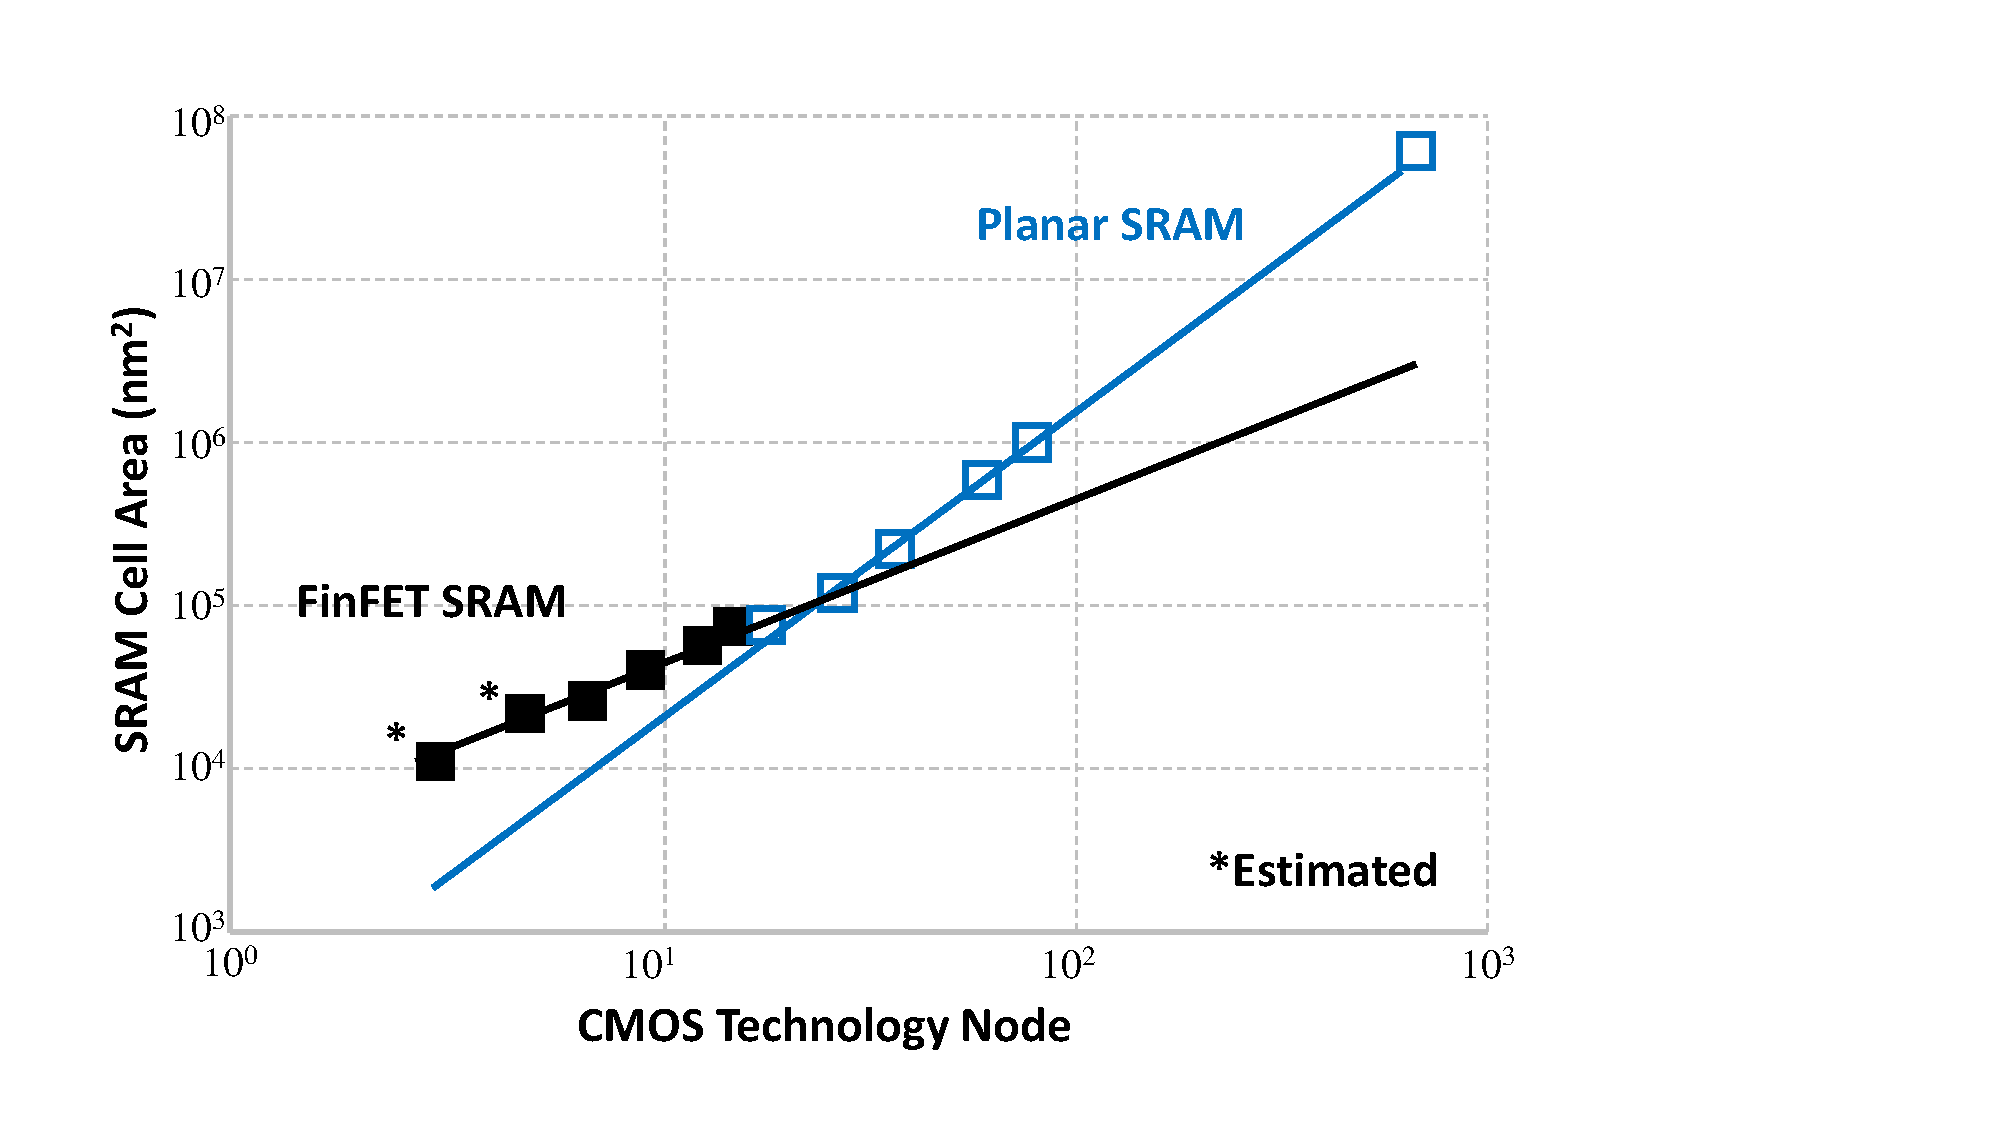
\includegraphics[width=0.8\linewidth]{Figures/example_plot.pdf}
    \caption{Here is an example figure}
    \label{fig:myfigure}
\end{figure}

%----------THESIS CONTENT-------------%
%-------------------------------------%
\chapter{Thesis Content}
\guide{thesisContent}

\begin{table}[h!]
    \centering
    \caption{Here is an example table.}
    \label{tbl:mytable}
    \begin{tabular}{c|c}

         something & something \\
         \hline
         something & something
    \end{tabular}
\end{table}


%----------SUMMARY--------------------%
%-------------------------------------%
\chapter{Summary and Conclusions}
\label{sec_conclusions}

\guide{thesisSummary}


%----------BIBLIOGRAPHY---------------%
%-------------------------------------%
%%%%%%%%%%%%%%%%%%%%%%%%%%%%%%%%%%%%%%%%%%%%%%%%%%%%%%%%%%%%%
%    This file configures your bibliography
%        Just a bit cleaner than having a long list of bib
%          files in your main document
%%%%%%%%%%%%%%%%%%%%%%%%%%%%%%%%%%%%%%%%%%%%%%%%%%%%%%%%%%%%%

% Start by defining the bibliography style
%    Some commonly used styles:
%       IEEEtran    - for most IEEE Transactions and Conference Proceedings
\ifacmjournal
    \bibliographystyle{ACM-Reference-Format}
\else
    \ifmicro
        \bibliographystyle{IEEEtranS}
    \else
        \bibliographystyle{IEEEtran}
    \fi
\fi


% A fresh manuscript with no citations yet produces an empty bibliography. The standard
% classes only warn about that, but IEEEtran stops with "perhaps a missing \item".
% Make every class just warn, so a freshly started paper always compiles.
% (Skipped for old-style classes such as sig-alternate that define no \endthebibliography.)
\makeatletter
\@ifundefined{endthebibliography}{}{%
    \let\enics@endthebibliography\endthebibliography
    \def\endthebibliography{%
        \def\@noitemerr{\@latex@warning{Empty thebibliography environment (no citations yet)}}%
        \enics@endthebibliography}%
}
\makeatother

% Now provide a list of bibliography files to include within the \bibliography command
%   These files are stored in the "bibliography" folder:
%     abbreviations.bib     - long and short names for common journals and conferences
%                             (use them as booktitle=ISCAS, journal=JSSC)
%     general_biblography   - things we tend to cite a lot (e.g., ITRS, textbooks, Moore's law)
%     <staff>_bibliography  - papers published by each of the EnICS staff members
%     this_bibliography.bib - put your paper-specific citations here!
%   BibTeX only prints the entries you actually cite, so loading all of them costs nothing.
\bibliography{bibliography/abbreviations,
              bibliography/general_biblography,
              bibliography/teman_bibliography,
              bibliography/fish_bibliography,
              bibliography/shor_bibliography,
              bibliography/itamar_bibliography,
              bibliography/osnat_bibliography,
              bibliography/yavits_bibliography,
              bibliography/this_bibliography}


%------HEBREW ABSTRACT---------%
%------------------------------%
\backmatter
\pagestyle{empty}
\ifluatex
    % Write your Hebrew abstract in AuxiliaryPages/abstract_hebrew.tex
    % Hebrew abstract (תקציר) for theses and research proposals.
% Write your Hebrew abstract in this file, replacing the guidance below.
% Requires LuaLaTeX (see AuxiliaryPages/hebrew_setup.tex).
\begin{otherlanguage}{hebrew}
\thispagestyle{empty}
\begin{center}
    {\LARGE\bfseries תקציר\par}
\end{center}
\vspace{1cm}
\noindent
\begin{guidance}
\guidenote{לכתוב פה תקציר לעבודה.
לוודא שהתקציר בעברית תואם את התקציר באנגלית!
להקפיד לסיים עם הישגי התיזה (למשל כמה מאמרים פורסמו על סמך המחקר).}
\end{guidance}
\end{otherlanguage}
\clearpage

\else
    % pdfLaTeX fallback: create the PDF from AuxiliaryPages/abstract_hebrew.docx
    
\includepdf[fitpaper,pages=-,pagecommand={}]{AuxiliaryPages/abstract_hebrew_example}
    \clearpage
\fi

%------HEBREW FRONT PAGES------%
%------------------------------%
\ifluatex
    % Hebrew table of contents, supervisor page and two Hebrew title pages,
    % from AuxiliaryPages/front_page_hebrew_phd.tex
    % Hebrew back matter for a PhD thesis (BIU Faculty of Engineering).
% The thesis is read from the back in Hebrew, so the order here is:
%   1. Hebrew table of contents (chapter titles in Hebrew; edit the list below)
%   2. Supervisor page
%   3. Hebrew title page for the inner cover
%   4. Identical Hebrew title page for the hard cover (the very last page)
% Fill in \thesisTitleHebrew, \thesisAuthorHebrew, \thesisAdvisorHebrew and \thesisDateHebrew in main.tex.
% Requires LuaLaTeX (see AuxiliaryPages/hebrew_setup.tex).
\newcommand{\phdHebrewTitlePage}{%
\thispagestyle{empty}
\begin{center}
    \vspace*{1cm}
    
\includegraphics[width=0.35\textwidth]{AuxiliaryPages/logos/biu_logo_hebrew}\par
    \vspace{1.5cm}
    {\Huge \thesisTitleHebrew\par}
    \vspace{2.5cm}
    {\Large חיבור לשם קבלת תואר "דוקטור לפילוסופיה"\par}
    \vspace{1cm}
    {\Large מאת:\par}
    \vspace{0.5em}
    {\LARGE\bfseries \thesisAuthorHebrew\par}
    \vspace{2.5cm}
    {\LARGE הפקולטה להנדסה\par}
    \vspace{2cm}
    {\LARGE הוגש לסנט של אוניברסיטת בר-אילן\par}
    \vfill
    {\Large רמת גן \hfill \thesisDateHebrew\par}
    \vspace{1cm}
\end{center}
\clearpage
}

\begin{otherlanguage}{hebrew}
%---- 1. Hebrew table of contents ----%
\thispagestyle{empty}
\vspace*{1cm}
{\LARGE\noindent\underline{תוכן עניינים:}\par}
\vspace{1em}
{\large\noindent
    פרק א': שם של פרק א' \dotfill\ 1\\
    פרק ב': שם של פרק ב' \dotfill\ 10\\
    פרק ג': שם של פרק ג' \dotfill\ 20\\
    פרק ד': שם של פרק ד' \dotfill\ 100\\
    פרק ה': שם של פרק ה' \dotfill\ 150\par}
\clearpage

%---- 2. Supervisor page ----%
\thispagestyle{empty}
\vspace*{2cm}
{\Large\noindent
    עבודה זו נעשתה בהדרכתו/ה של \thesisAdvisorHebrew\\[0.5em]
    מן הפקולטה להנדסה של אוניברסיטת בר-אילן\par}
\clearpage

%---- 3 and 4. Title pages ----%
\phdHebrewTitlePage
\phdHebrewTitlePage
\end{otherlanguage}

\else
    % pdfLaTeX fallback: create the PDF from AuxiliaryPages/front_page_hebrew_phd_thesis.docx
    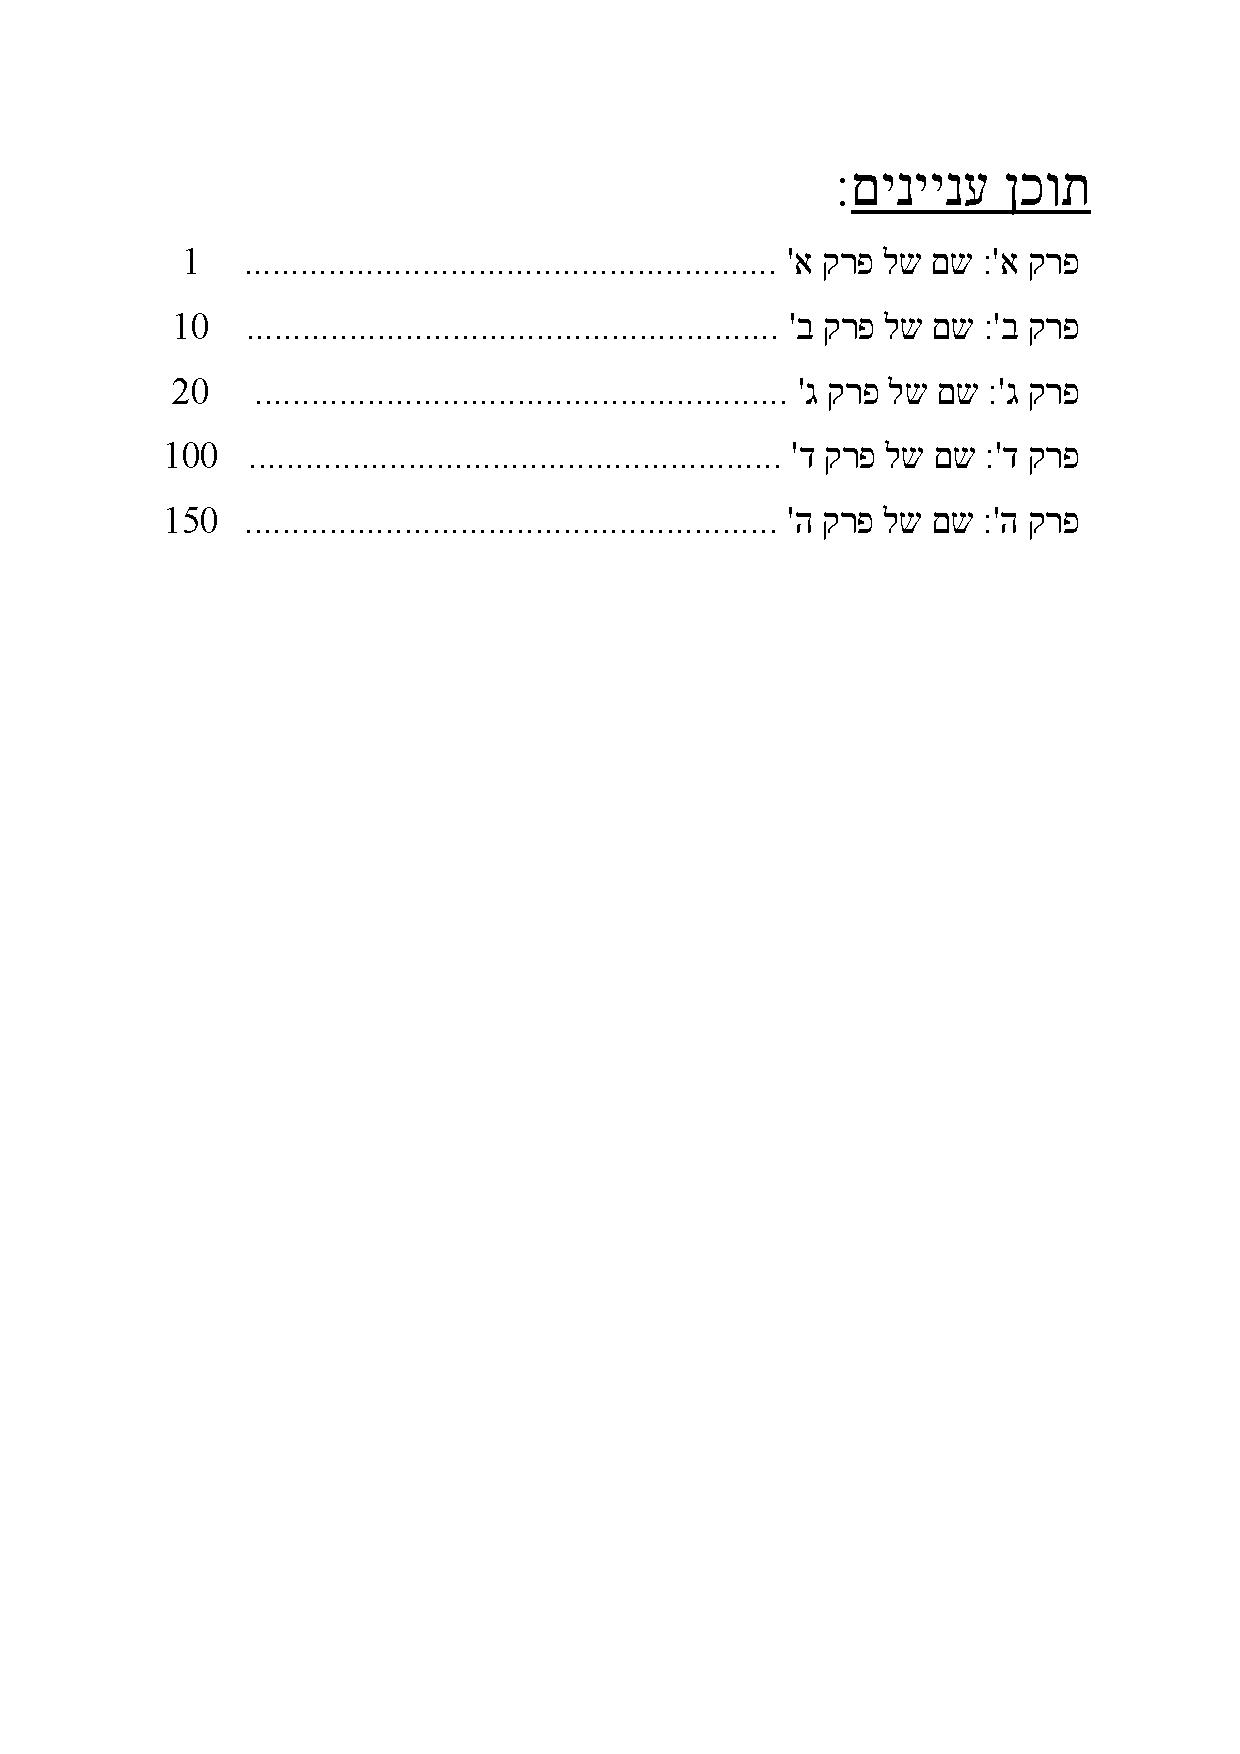
\includepdf[fitpaper,pages=-,pagecommand={}]{AuxiliaryPages/front_page_hebrew_phd_thesis_example}
    \clearpage
\fi


\end{document}


% For Research Proposal (compile with LuaLaTeX for the Hebrew pages)
% \documentclass[a4paper,12pt]{article}
%%%%%%%%%%%%%%%%%%%%%%%%%%%%%%%%%%%%%%%%%%%%%%%%%%%%%%%%%%%%%%%%%%%%%%%%%%%
%   EnICS Templates: MSc / PhD Research Proposal (Bar-Ilan University)
%   To start writing: make this file the main.tex in the root of the project
%   (see README.md, or ask Claude to "start a new EnICS manuscript").
%
%   Compile with LuaLaTeX (Overleaf: Menu --> Compiler --> LuaLaTeX) to get the
%   Hebrew front page and the Hebrew abstract typeset directly from the .tex
%   files under AuxiliaryPages. With pdfLaTeX, they fall back to PDFs that you
%   create from the .docx files under AuxiliaryPages.
%%%%%%%%%%%%%%%%%%%%%%%%%%%%%%%%%%%%%%%%%%%%%%%%%%%%%%%%%%%%%%%%%%%%%%%%%%%

%%%%%%%%%%%%%%%%%%%%%%%%%%%%%%%%%%%%%%%%%%%%%
%    EnICS Templates: version stamp
%%%%%%%%%%%%%%%%%%%%%%%%%%%%%%%%%%%%%%%%%%%%%
% Bump this when releasing a new version of the templates to GitHub.
% Derived projects carry it, so anyone can tell which template version they started from.
\newcommand{\enicstemplateversion}{2026.09}

%%%%%%%%%%%%%%%%%%%%%%%%%%%%%%%%%%%%%%%%%%%%%
%    Don't warn me about loading packages
%%%%%%%%%%%%%%%%%%%%%%%%%%%%%%%%%%%%%%%%%%%%%
\usepackage{silence}

%%%%%%%%%%%%%%%%%%%%%%%%%%%%%%%%%%%%%%%%%%%%%
%    Template guidance switch
%%%%%%%%%%%%%%%%%%%%%%%%%%%%%%%%%%%%%%%%%%%%%
% All explanatory (colored) text in the templates is conditional on \ifguide.
% Each template sets \guidetrue in its preamble; change it to \guidefalse
% to remove every piece of guidance from the PDF at once.
\newif\ifguide
    \guidetrue

%%%%%%%%%%%%%%%%%%%%%%%%%%%%%%%%%%%%%%%%%%%%%
%    Variables per conference/journal
%%%%%%%%%%%%%%%%%%%%%%%%%%%%%%%%%%%%%%%%%%%%%
% All variables are false by default. Each template turns on the one(s) it needs.

% For Research Proposal template specific configurations
\newif\ifproposal
    \proposalfalse

% For Thesis template specific configurations
\newif\ifthesis
    \thesisfalse

% For IEEE Journal template specific configurations
\newif\ifieeejournal
    \ieeejournalfalse
% For ACM Journal template specific configurations
%     based on the template found here: https://www.acm.org/publications/authors/submissions
\newif\ifacmjournal
    \acmjournalfalse
% For adding author biographies
\newif\ifbiographies
    \biographiesfalse
% For adding a reply to reviewers
\newif\ifreplytoreviewers
    \replytoreviewersfalse

% For IEEE Conference template specific configurations
\newif\ifieeeconference
    \ieeeconferencefalse

% For ISF template specific configurations
\newif\ifisf
    \isffalse

% For ACM Conference (MICRO) template specific configurations
\newif\ifmicro
    \microfalse

% For template specific configurations
% \newif\if
%     \false

    \proposaltrue           % Research Proposal specific configurations
    \guidetrue              % Show the template guidance text. Change to \guidefalse to hide all of it.

\usepackage{packages/basic_packages}
\input{packages/macros}
\input{newcommands/units}
%=================================%
% 	    	GLOSSARY       	      %
%   Common Acronyms & Commands    %
%=================================%
% \gls{formula}   -> singular -> e.g: formula 
% \Gls{formula}   -> singular + capital letter -> e.g: Formula 
% \glspl{formula} -> plural -> e.g: formulas 
% \Glspl{formula} -> plural + capital letter -> e.g: Formula
%
%   \newacronym{}{}{}
%   \newcommand{\}{}
\newacronym{sota}{SoTA}{state-of-the-art}
    \newcommand{\sota}{\gls{sota}\xspace}
\newacronym{iot}{IoT}{internet-of-things}
    \newcommand{\iot}{\gls{iot}\xspace} 
    \newcommand{\Iot}{\Gls{iot}\xspace} 
\newacronym{snr}{SNR}{signal-to-noise ratio}
    \newcommand{\snr}{\gls{snr}\xspace}
\newacronym{ppa}{PPA}{performance, power, and area}
    \newcommand{\ppa}{\gls{ppa}\xspace}
\newcommand{\var}{$\sigma/\mu$\xspace}
\newcommand{\std}{$\sigma$\xspace}

\newacronym{cdf}{CDF}{cumulative distribution function}
\newacronym{pdf}{PDF}{probabililty distribution function}
\newacronym{ip}{IP}{intellectual property}
\newacronym{fir}{FIR}{finite impulse response}
\newacronym{dsp}{DSP}{digital signal processing}
\newacronym[longplural={central processing units}]{cpu}{CPU}{central processing unit}
    \newcommand{\cpu}{\gls{cpu}\xspace} 
    \newcommand{\Cpu}{\Gls{cpu}\xspace} 
    \newcommand{\cpus}{\glspl{cpu}\xspace}
    \newcommand{\Cpus}{\Glspl{cpu}\xspace}
    
\input{newcommands/enics_glossary}
\input{newcommands/vlsi_glossary}
\newacronym{ai}{AI}{artificial-intelligence}
    \newcommand{\ai}{\gls{ai}\xspace} 
    \newcommand{\Ai}{\Gls{ai}\xspace} 
\newacronym{ml}{ML}{machine learning}
    \newcommand{\ml}{\gls{ml}\xspace}
\newacronym{mac}{MAC}{multiply-and-accumulate}
    \newcommand{\mac}{\gls{mac}\xspace}
    \newcommand{\macs}{\glspl{mac}\xspace}
\newacronym{dl}{DL}{deep learning}
    \newcommand{\dl}{\gls{dl}\xspace}
\newacronym{cnn}{CNN}{convolutional neural network}
    \newcommand{\cnn}{\gls{cnn}\xspace}
\newacronym{dnn}{DNN}{deep neural network}
    \newcommand{\dnn}{\gls{dnn}\xspace}
    \newcommand{\dnns}{\glspl{dnn}\xspace}
\newacronym[longplural={graphic processing units}]{gpu}{GPU}{graphic processing unit}
    \newcommand{\gpu}{\gls{gpu}\xspace} 
    \newcommand{\Gpu}{\Gls{gpu}\xspace} 
    \newcommand{\gpus}{\glspl{gpu}\xspace}
    \newcommand{\Gpus}{\Glspl{gpu}\xspace}
\newacronym{vit}{ViT}{vision transformer}
    \newcommand{\vit}{\gls{vit}\xspace}
\newacronym{tpu}{TPU}{tensor processing unit}
    \newcommand{\tpu}{\gls{tpu}\xspace}
\newacronym{relu}{ReLu}{rectified linear unit}
    \newcommand{\relu}{\gls{relu}\xspace}
\newacronym{llm}{LLM}{Large Language Model}
    \newcommand{\llm}{\gls{llm}\xspace}
    \newcommand{\llms}{\glspl{llm}\xspace}
\newacronym{AF}{AF}{activation function}
    \newcommand{\AF}{\gls{AF}\xspace}
    \newcommand{\AFs}{\glspl{AF}\xspace}

\newacronym{cordic}{CORDIC}{COordinate Rotation DIgital Computer}
    \newcommand{\cordic}{\gls{cordic}\xspace}

\newcommand{\softmax}{SoftMax\xspace}
%\newcommand{\relu}{ReLu\xspace}
\newcommand{\selu}{SeLu\xspace}
\newcommand{\gelu}{GeLu\xspace}

\newacronym{fsm}{FSM}{finite state machine}
    \newcommand{\fsm}{\gls{fsm}\xspace}
    \newcommand{\fsms}{\glspl{fsm}\xspace}

% \newacronym{lut}{LUT}{Look-Up Table}
     \newcommand{\lut}{\gls{lut}\xspace}
     \newcommand{\luts}{\glspl{lut}\xspace}


\newacronym{PE}{PE}{processing element}
    \newcommand{\PE}{\gls{PE}\xspace}
    \newcommand{\PEs}{\glspl{PE}\xspace}

\newacronym{RNN}{RNN}{recurrent neural networks}
    \newcommand{\RNN}{\gls{RNN}\xspace}
    \newcommand{\RNNs}{\glspl{RNN}\xspace}

\newacronym{QAT}{QAT}{quantization-aware training}
     \newcommand{\QAT}{\gls{QAT}\xspace}
\newacronym{short}{PTQ}{post-training quantization}
     \newcommand{\PTQ}{\gls{PTQ}\xspace}
% This is where you should define proposal-specific newcommands and acronyms
\input{newcommands/this_glossary}

%%%%%%%%%%%%%%%%%%%%%%%%%%%%%%%%%%%%%%%
%          PROPOSAL DETAILS           %
%   (used by the Hebrew front page under AuxiliaryPages)
%%%%%%%%%%%%%%%%%%%%%%%%%%%%%%%%%%%%%%%
\newcommand{\proposalTitle}{Research Title}
\newcommand{\proposalAuthor}{First Name Last Name}
% Hebrew details (typeset only when compiling with LuaLaTeX)
\newcommand{\proposalDegreeHebrew}{שלישי}          % שלישי for PhD, שני for MSc
\newcommand{\proposalTitleHebrew}{כותרת המחקר בעברית}
\newcommand{\proposalAuthorHebrew}{שם המגיש/ה}
\newcommand{\proposalAuthorID}{תעודת זהות}
\newcommand{\proposalAdvisorHebrew}{שם המנחה}

\title{\proposalTitle}
\author{\proposalAuthor}
\date{}


%%%%%%%%%%%%%%%%%%%%%%%%%%%%%%%%%%%%%%%
%           DOCUMENT BEGINS           %
%%%%%%%%%%%%%%%%%%%%%%%%%%%%%%%%%%%%%%%
\begin{document}

%-----Hebrew Front Page------------%
%----------------------------------%
\ifluatex
    % Hebrew front page for a research proposal (BIU Faculty of Engineering).
% Fill in \proposalTitle, \proposalTitleHebrew, \proposalAuthorHebrew, \proposalAuthorID,
% \proposalAdvisorHebrew and \proposalDegreeHebrew in main.tex.
% Requires LuaLaTeX (see AuxiliaryPages/hebrew_setup.tex).
\begin{otherlanguage}{hebrew}
\thispagestyle{empty}
\begin{center}
    \vspace*{1cm}
    
\includegraphics[width=0.35\textwidth]{AuxiliaryPages/logos/biu_logo_hebrew_proposal}\par
    \vspace{0.5em}
    {\Large הפקולטה להנדסה\par}
    \vspace{2.5cm}
    {\fontsize{32}{40}\selectfont הצעת מחקר לתואר \proposalDegreeHebrew\par}
    \vspace{2cm}
\end{center}
{\large\noindent\bfseries הנושא:\par}
\begin{center}
    \vspace{0.5em}
    {\Large\bfseries \proposalTitleHebrew\par}
    \vspace{1.5em}
    {\Large\bfseries \proposalTitle\par}
    \vspace{3cm}
    {\Large שם המנחה: \proposalAdvisorHebrew\par}
    \vspace{1.5cm}
    {\Large \proposalAuthorHebrew \quad \proposalAuthorID\par}
\end{center}
\end{otherlanguage}
\clearpage

\else
    % pdfLaTeX fallback: create the PDF from AuxiliaryPages/front_page_hebrew_phd_proposal.docx
    \thispagestyle{empty}
    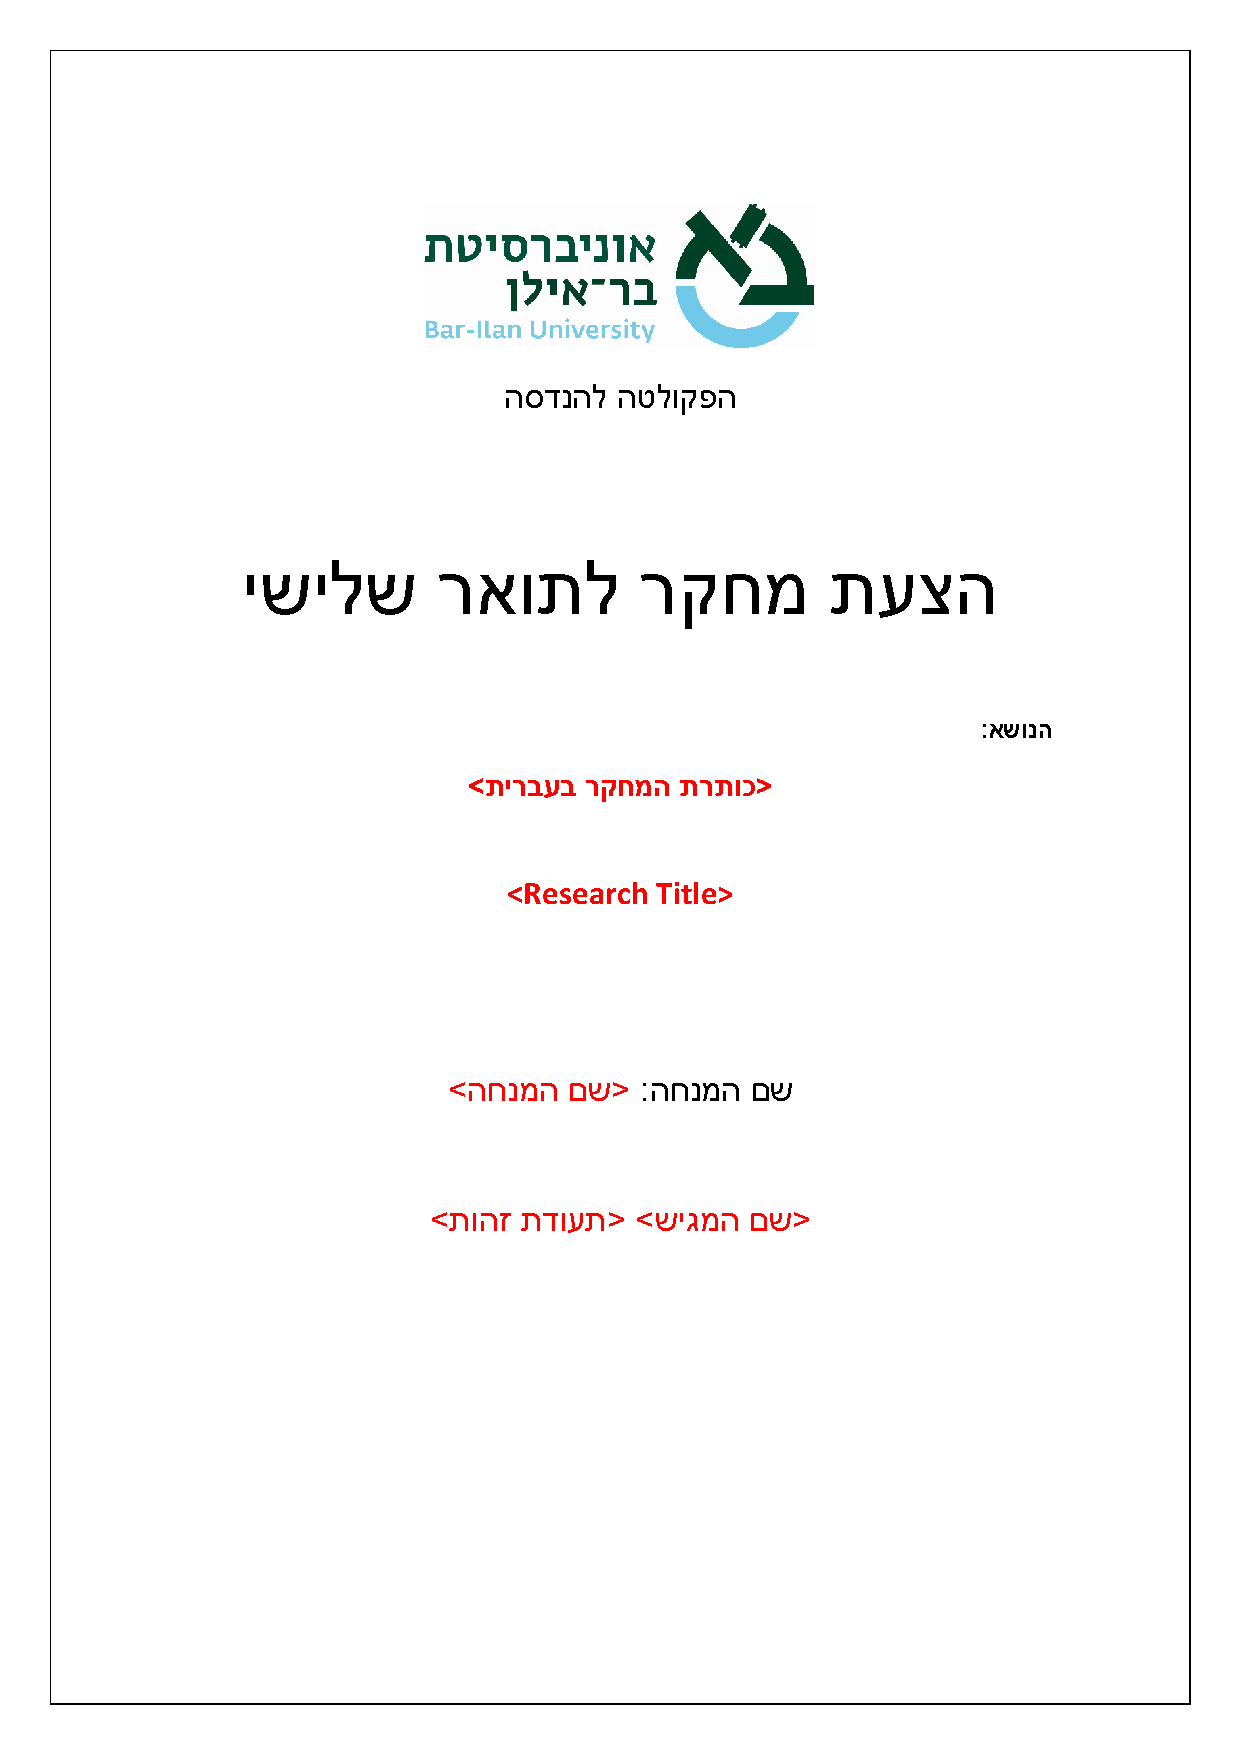
\includepdf[fitpaper,pages=-,pagecommand={}]{AuxiliaryPages/front_page_hebrew_phd_proposal_example}
    \clearpage
\fi


%----------ABSTRACT-------------------%
%-------------------------------------%
\section*{Abstract}
    \guide{abstractRP}
\clearpage


\glsresetall

%-----Hebrew Abstract--------------%
%----------------------------------%
\ifluatex
    % Write your Hebrew abstract in AuxiliaryPages/abstract_hebrew.tex
    % Hebrew abstract (תקציר) for theses and research proposals.
% Write your Hebrew abstract in this file, replacing the guidance below.
% Requires LuaLaTeX (see AuxiliaryPages/hebrew_setup.tex).
\begin{otherlanguage}{hebrew}
\thispagestyle{empty}
\begin{center}
    {\LARGE\bfseries תקציר\par}
\end{center}
\vspace{1cm}
\noindent
\begin{guidance}
\guidenote{לכתוב פה תקציר לעבודה.
לוודא שהתקציר בעברית תואם את התקציר באנגלית!
להקפיד לסיים עם הישגי התיזה (למשל כמה מאמרים פורסמו על סמך המחקר).}
\end{guidance}
\end{otherlanguage}
\clearpage

\else
    % pdfLaTeX fallback: create the PDF from AuxiliaryPages/abstract_hebrew.docx
    
\includepdf[fitpaper,pages=-,pagecommand={\thispagestyle{plain}}]{AuxiliaryPages/abstract_hebrew_example}
    \clearpage
\fi

%-----Table of Contents------------%
%----------------------------------%
    \tableofcontents
\clearpage

%-----List of Figures--------------%
%----------------------------------%
    \listoffigures
\clearpage



%----------INTRODUCTION---------------%
%-------------------------------------%
\section{Introduction}
\label{sec_intro}

This is the introduction section.

\clearpage

%----------BACKGROUND-----------------%
%-------------------------------------%
\section{Background}
\label{sec_background}

This is the background section.

\clearpage

%-------RESEARCH OBJECTIVES-----------%
%-------------------------------------%
\section{Research Objective and Methodology}
\subsection{Objectives}
    \label{sec_objectives}
    \guide{objectives}

\subsection{Methodology}
    \label{sec_methodology}
    \guide{methodology}

\clearpage

%-------PRELIMINARY RESULTS-----------%
%-------------------------------------%
\section{Preliminary Results}
\clearpage

%----------BIBLIOGRAPHY---------------%
%-------------------------------------%
%%%%%%%%%%%%%%%%%%%%%%%%%%%%%%%%%%%%%%%%%%%%%%%%%%%%%%%%%%%%%
%    This file configures your bibliography
%        Just a bit cleaner than having a long list of bib
%          files in your main document
%%%%%%%%%%%%%%%%%%%%%%%%%%%%%%%%%%%%%%%%%%%%%%%%%%%%%%%%%%%%%

% Start by defining the bibliography style
%    Some commonly used styles:
%       IEEEtran    - for most IEEE Transactions and Conference Proceedings
\ifacmjournal
    \bibliographystyle{ACM-Reference-Format}
\else
    \ifmicro
        \bibliographystyle{IEEEtranS}
    \else
        \bibliographystyle{IEEEtran}
    \fi
\fi


% A fresh manuscript with no citations yet produces an empty bibliography. The standard
% classes only warn about that, but IEEEtran stops with "perhaps a missing \item".
% Make every class just warn, so a freshly started paper always compiles.
% (Skipped for old-style classes such as sig-alternate that define no \endthebibliography.)
\makeatletter
\@ifundefined{endthebibliography}{}{%
    \let\enics@endthebibliography\endthebibliography
    \def\endthebibliography{%
        \def\@noitemerr{\@latex@warning{Empty thebibliography environment (no citations yet)}}%
        \enics@endthebibliography}%
}
\makeatother

% Now provide a list of bibliography files to include within the \bibliography command
%   These files are stored in the "bibliography" folder:
%     abbreviations.bib     - long and short names for common journals and conferences
%                             (use them as booktitle=ISCAS, journal=JSSC)
%     general_biblography   - things we tend to cite a lot (e.g., ITRS, textbooks, Moore's law)
%     <staff>_bibliography  - papers published by each of the EnICS staff members
%     this_bibliography.bib - put your paper-specific citations here!
%   BibTeX only prints the entries you actually cite, so loading all of them costs nothing.
\bibliography{bibliography/abbreviations,
              bibliography/general_biblography,
              bibliography/teman_bibliography,
              bibliography/fish_bibliography,
              bibliography/shor_bibliography,
              bibliography/itamar_bibliography,
              bibliography/osnat_bibliography,
              bibliography/yavits_bibliography,
              bibliography/this_bibliography}


\end{document}


% For ISF Proposal
% %%%%%%%%%%%%%%%%%%%%%%%%%%%%%%%%%%%%%%%%%%%%%%%%%%%%%%%%%%%%%%%%%%%%%%%%%%%
%   EnICS Templates: ISF (Israel Science Foundation) Regular Program proposal
%   To start writing: make this file the main.tex in the root of the project
%   (see README.md, or ask Claude to "start a new EnICS manuscript").
%
%   ISF rules (check the current call!):
%     File format - Doc or PDF only
%     Sections (all in one file):
%       Research program - up to 10 A4 pages
%       Figures - up to 5 A4 pages
%       Bibliography - up to 5 A4 pages
%     In the bibliography included in the research plan file, do not mark * for the
%     articles that are more relevant to the application. A separate bibliography file
%     including * should be uploaded in the attached file section.
%     All parts should be typed in standard font size (Times new Roman or Arial size 11),
%     with a line spacing 1.5.
%%%%%%%%%%%%%%%%%%%%%%%%%%%%%%%%%%%%%%%%%%%%%%%%%%%%%%%%%%%%%%%%%%%%%%%%%%%
\documentclass[a4paper,11pt]{article}

%%%%%%%%%%%%%%%%%%%%%%%%%%%%%%%%%%%%%%%%%%%%%
%    EnICS Templates: version stamp
%%%%%%%%%%%%%%%%%%%%%%%%%%%%%%%%%%%%%%%%%%%%%
% Bump this when releasing a new version of the templates to GitHub.
% Derived projects carry it, so anyone can tell which template version they started from.
\newcommand{\enicstemplateversion}{2026.09}

%%%%%%%%%%%%%%%%%%%%%%%%%%%%%%%%%%%%%%%%%%%%%
%    Don't warn me about loading packages
%%%%%%%%%%%%%%%%%%%%%%%%%%%%%%%%%%%%%%%%%%%%%
\usepackage{silence}

%%%%%%%%%%%%%%%%%%%%%%%%%%%%%%%%%%%%%%%%%%%%%
%    Template guidance switch
%%%%%%%%%%%%%%%%%%%%%%%%%%%%%%%%%%%%%%%%%%%%%
% All explanatory (colored) text in the templates is conditional on \ifguide.
% Each template sets \guidetrue in its preamble; change it to \guidefalse
% to remove every piece of guidance from the PDF at once.
\newif\ifguide
    \guidetrue

%%%%%%%%%%%%%%%%%%%%%%%%%%%%%%%%%%%%%%%%%%%%%
%    Variables per conference/journal
%%%%%%%%%%%%%%%%%%%%%%%%%%%%%%%%%%%%%%%%%%%%%
% All variables are false by default. Each template turns on the one(s) it needs.

% For Research Proposal template specific configurations
\newif\ifproposal
    \proposalfalse

% For Thesis template specific configurations
\newif\ifthesis
    \thesisfalse

% For IEEE Journal template specific configurations
\newif\ifieeejournal
    \ieeejournalfalse
% For ACM Journal template specific configurations
%     based on the template found here: https://www.acm.org/publications/authors/submissions
\newif\ifacmjournal
    \acmjournalfalse
% For adding author biographies
\newif\ifbiographies
    \biographiesfalse
% For adding a reply to reviewers
\newif\ifreplytoreviewers
    \replytoreviewersfalse

% For IEEE Conference template specific configurations
\newif\ifieeeconference
    \ieeeconferencefalse

% For ISF template specific configurations
\newif\ifisf
    \isffalse

% For ACM Conference (MICRO) template specific configurations
\newif\ifmicro
    \microfalse

% For template specific configurations
% \newif\if
%     \false

    \isftrue                % ISF specific configurations
    \guidetrue              % Show the template guidance text. Change to \guidefalse to hide all of it.

\usepackage{packages/basic_packages}
\input{packages/macros}
\input{newcommands/units}
%=================================%
% 	    	GLOSSARY       	      %
%   Common Acronyms & Commands    %
%=================================%
% \gls{formula}   -> singular -> e.g: formula 
% \Gls{formula}   -> singular + capital letter -> e.g: Formula 
% \glspl{formula} -> plural -> e.g: formulas 
% \Glspl{formula} -> plural + capital letter -> e.g: Formula
%
%   \newacronym{}{}{}
%   \newcommand{\}{}
\newacronym{sota}{SoTA}{state-of-the-art}
    \newcommand{\sota}{\gls{sota}\xspace}
\newacronym{iot}{IoT}{internet-of-things}
    \newcommand{\iot}{\gls{iot}\xspace} 
    \newcommand{\Iot}{\Gls{iot}\xspace} 
\newacronym{snr}{SNR}{signal-to-noise ratio}
    \newcommand{\snr}{\gls{snr}\xspace}
\newacronym{ppa}{PPA}{performance, power, and area}
    \newcommand{\ppa}{\gls{ppa}\xspace}
\newcommand{\var}{$\sigma/\mu$\xspace}
\newcommand{\std}{$\sigma$\xspace}

\newacronym{cdf}{CDF}{cumulative distribution function}
\newacronym{pdf}{PDF}{probabililty distribution function}
\newacronym{ip}{IP}{intellectual property}
\newacronym{fir}{FIR}{finite impulse response}
\newacronym{dsp}{DSP}{digital signal processing}
\newacronym[longplural={central processing units}]{cpu}{CPU}{central processing unit}
    \newcommand{\cpu}{\gls{cpu}\xspace} 
    \newcommand{\Cpu}{\Gls{cpu}\xspace} 
    \newcommand{\cpus}{\glspl{cpu}\xspace}
    \newcommand{\Cpus}{\Glspl{cpu}\xspace}
    
\input{newcommands/enics_glossary}
\input{newcommands/vlsi_glossary}
\newacronym{ai}{AI}{artificial-intelligence}
    \newcommand{\ai}{\gls{ai}\xspace} 
    \newcommand{\Ai}{\Gls{ai}\xspace} 
\newacronym{ml}{ML}{machine learning}
    \newcommand{\ml}{\gls{ml}\xspace}
\newacronym{mac}{MAC}{multiply-and-accumulate}
    \newcommand{\mac}{\gls{mac}\xspace}
    \newcommand{\macs}{\glspl{mac}\xspace}
\newacronym{dl}{DL}{deep learning}
    \newcommand{\dl}{\gls{dl}\xspace}
\newacronym{cnn}{CNN}{convolutional neural network}
    \newcommand{\cnn}{\gls{cnn}\xspace}
\newacronym{dnn}{DNN}{deep neural network}
    \newcommand{\dnn}{\gls{dnn}\xspace}
    \newcommand{\dnns}{\glspl{dnn}\xspace}
\newacronym[longplural={graphic processing units}]{gpu}{GPU}{graphic processing unit}
    \newcommand{\gpu}{\gls{gpu}\xspace} 
    \newcommand{\Gpu}{\Gls{gpu}\xspace} 
    \newcommand{\gpus}{\glspl{gpu}\xspace}
    \newcommand{\Gpus}{\Glspl{gpu}\xspace}
\newacronym{vit}{ViT}{vision transformer}
    \newcommand{\vit}{\gls{vit}\xspace}
\newacronym{tpu}{TPU}{tensor processing unit}
    \newcommand{\tpu}{\gls{tpu}\xspace}
\newacronym{relu}{ReLu}{rectified linear unit}
    \newcommand{\relu}{\gls{relu}\xspace}
\newacronym{llm}{LLM}{Large Language Model}
    \newcommand{\llm}{\gls{llm}\xspace}
    \newcommand{\llms}{\glspl{llm}\xspace}
\newacronym{AF}{AF}{activation function}
    \newcommand{\AF}{\gls{AF}\xspace}
    \newcommand{\AFs}{\glspl{AF}\xspace}

\newacronym{cordic}{CORDIC}{COordinate Rotation DIgital Computer}
    \newcommand{\cordic}{\gls{cordic}\xspace}

\newcommand{\softmax}{SoftMax\xspace}
%\newcommand{\relu}{ReLu\xspace}
\newcommand{\selu}{SeLu\xspace}
\newcommand{\gelu}{GeLu\xspace}

\newacronym{fsm}{FSM}{finite state machine}
    \newcommand{\fsm}{\gls{fsm}\xspace}
    \newcommand{\fsms}{\glspl{fsm}\xspace}

% \newacronym{lut}{LUT}{Look-Up Table}
     \newcommand{\lut}{\gls{lut}\xspace}
     \newcommand{\luts}{\glspl{lut}\xspace}


\newacronym{PE}{PE}{processing element}
    \newcommand{\PE}{\gls{PE}\xspace}
    \newcommand{\PEs}{\glspl{PE}\xspace}

\newacronym{RNN}{RNN}{recurrent neural networks}
    \newcommand{\RNN}{\gls{RNN}\xspace}
    \newcommand{\RNNs}{\glspl{RNN}\xspace}

\newacronym{QAT}{QAT}{quantization-aware training}
     \newcommand{\QAT}{\gls{QAT}\xspace}
\newacronym{short}{PTQ}{post-training quantization}
     \newcommand{\PTQ}{\gls{PTQ}\xspace}
\input{newcommands/this_glossary}


% Insert in the header of the file the application no. & the first PI's name, aligned to the right.
\rhead{Application No. XXX/XX \\
            PI Name: XXX XXXX}
\def \mytitle {EnICS ISF Proposal Template}

\title{\mytitle}
\author{}
\date{}

\begin{document}

%%%%%%%%%%%%%%%%%%%%%%%%%%%%%%%%%%%%%%%%%%%%%
%  Scientific Abstract
%%%%%%%%%%%%%%%%%%%%%%%%%%%%%%%%%%%%%%%%%%%%%


\noindent\textsf{\underline{Scientific Abstract}:}

\section*{\centering Write the title here }

The scientific abstract of the proposal

\newpage

%%%%%%%%%%%%%%%%%%%%%%%%%%%%%%%%%%%%%%%%%%%%%
%  Proposal
%%%%%%%%%%%%%%%%%%%%%%%%%%%%%%%%%%%%%%%%%%%%%


\Large\textsf{\\\underline{Detailed description of the research program}\\}
\normalsize

\section*{\vspace{-5px}\centering\LARGE   Write the title here}
%\vspace{5mm}

%Research program - up to 10 A4 pages
\section{Scientific Background}
\label{sec:scientific_background}

% -----------------------------------------------------------------------------
\subsection{Background and Introduction}\label{sec:stateofart:intro}
% -----------------------------------------------------------------------------
\guidenote{2.5 pages}

Some intro stuff
\\


Throughout my research career, I have focused on
\\

\noindent\textit{\textbf{Summary}}:
In this four year research, I propose to

\section{Research objectives and expected significance}
\label{sec:objectives}
\guidenote{1 page}

The main objective of this research is to
\\

\noindent Specifically, the proposed research has the following detailed objectives:
\begin{itemize}
    \item To develop
\end{itemize}

\section{Detailed description of the proposed research}
\guidenote{4.5 pages}

\subsection{Working hypothesis}
\label{sec:hypothesis}

\subsubsection{Something }

To summarize,

\subsection{Research design and methods}
\label{sec:methods}
\guidenote{1 page}

The proposed research objectives will be achieved by

In particular, this research will be carried out according to the following phases:
\begin{itemize}
    \item \underline{Phase 1}: The initial stage of this research
    \item \underline{Phase 2}: The second stage of this research
\end{itemize}

\subsection{Preliminary Results}
\label{sec:preliminary_results}
\guidenote{half a page}

The proposed research is based on the research I have carried out in recent years focusing on


\subsection{Equipment and Laboratory Setup for Proposed Research}
\label{sec:equipment}
\guidenote{half a page}


%%%%%%%%%%%%%%%%%%%%%%%%%%%%%%%%%%%%%%%%%%%%%
%  Bibliography
%%%%%%%%%%%%%%%%%%%%%%%%%%%%%%%%%%%%%%%%%%%%%
\newpage
\singlespacing
%%%%%%%%%%%%%%%%%%%%%%%%%%%%%%%%%%%%%%%%%%%%%%%%%%%%%%%%%%%%%
%    This file configures your bibliography
%        Just a bit cleaner than having a long list of bib
%          files in your main document
%%%%%%%%%%%%%%%%%%%%%%%%%%%%%%%%%%%%%%%%%%%%%%%%%%%%%%%%%%%%%

% Start by defining the bibliography style
%    Some commonly used styles:
%       IEEEtran    - for most IEEE Transactions and Conference Proceedings
\ifacmjournal
    \bibliographystyle{ACM-Reference-Format}
\else
    \ifmicro
        \bibliographystyle{IEEEtranS}
    \else
        \bibliographystyle{IEEEtran}
    \fi
\fi


% A fresh manuscript with no citations yet produces an empty bibliography. The standard
% classes only warn about that, but IEEEtran stops with "perhaps a missing \item".
% Make every class just warn, so a freshly started paper always compiles.
% (Skipped for old-style classes such as sig-alternate that define no \endthebibliography.)
\makeatletter
\@ifundefined{endthebibliography}{}{%
    \let\enics@endthebibliography\endthebibliography
    \def\endthebibliography{%
        \def\@noitemerr{\@latex@warning{Empty thebibliography environment (no citations yet)}}%
        \enics@endthebibliography}%
}
\makeatother

% Now provide a list of bibliography files to include within the \bibliography command
%   These files are stored in the "bibliography" folder:
%     abbreviations.bib     - long and short names for common journals and conferences
%                             (use them as booktitle=ISCAS, journal=JSSC)
%     general_biblography   - things we tend to cite a lot (e.g., ITRS, textbooks, Moore's law)
%     <staff>_bibliography  - papers published by each of the EnICS staff members
%     this_bibliography.bib - put your paper-specific citations here!
%   BibTeX only prints the entries you actually cite, so loading all of them costs nothing.
\bibliography{bibliography/abbreviations,
              bibliography/general_biblography,
              bibliography/teman_bibliography,
              bibliography/fish_bibliography,
              bibliography/shor_bibliography,
              bibliography/itamar_bibliography,
              bibliography/osnat_bibliography,
              bibliography/yavits_bibliography,
              bibliography/this_bibliography}


\end{document}

